\documentclass[14pt]{extreport}
\usepackage{listings}
\usepackage[english]{babel}
\usepackage[utf8]{inputenc}
\usepackage{amsmath}
\usepackage{graphicx}
\usepackage{textcomp}
\usepackage{float}
\usepackage[colorinlistoftodos]{todonotes}
\usepackage{hyperref}
\title{Data Mining}

\author{Luca Corbucci}

\date{\today}

\begin{document}
\maketitle

\tableofcontents

\chapter{Definizioni}

\begin{itemize}
\item Media: la somma dei valori che abbiamo divisa per il numero di valori;
\item Mediana: abbiamo una serie di dati, li disponiamo in ordine crescente (o decrescente) e poi prendiamo il valore che sta nel mezzo, questa è la mediana;
\item Moda: dato l'insieme di dati la moda è il valore che compare più di frequente;
\item q\%-quantile: è il valore che mi divide i dati in due parti una parte rappresenta il q\% dei valori e sono quelli minori del valore che ho scelto, l'altra parte è il 100-q\% dei valori e rappresenta i valori maggiori. Abbiamo ad esempio il primo quartile che è il 25\%, il secondo quartile è il 50\% e il terzo è il 75\% quartile.
\item Varianza: è una funzione che fornisce la misura della variabilità dei valori che sono assunti dalla variabile stessa. Ad esempio questa varianza mi indica quanto i valori si distaccano dalla media o dal valore atteso.
Due modi per stabilizzare la varianza:
\begin{itemize}
\item Logaritmica: 
\begin{equation}
T(x) = cLogx + d
\end{equation}
\item Quadratica:
\begin{equation}
T(x) = ax^p + b
\end{equation}
\end{itemize}
\item Normalizzazione di una distribuzione: procedimento che ci permette di limitare l'escursione di un insieme di valori entro un certo intervallo predefinito.
Ci sono due modi per fare la normalizzazione:
\begin{itemize}
\item Normalizzazione Min-Max: 
\begin{equation}
v' = \frac{v-min_a}{max_a - min_a} (newMax_a - newMin_a) + newMin_a
\end{equation}
\item Z-Score:
\begin{equation}
v' = \frac{v-mean_a}{stdDev_a}
\end{equation}
\end{itemize}
\end{itemize}

\chapter{Data Understanding}

Data una tabella abbiamo varie tipologie di attributi che possiamo trovare all'interno:
\begin{itemize}
\item Categorico: attributo che mi indica l'appartenenza ad una certa categoria, ad esempio maschio o femmina
\item Ordinale: attributo che indica l'appartenenza ad una categoria che però è ordinata rispetto ad altre categorie, ad esempio studente magistrale è un ordinale perchè è dopo studente triennale ma prima di dottorato.
\item Valori numerici
\item Valori discreti: sono un sottoinsieme dei valori interi
\item Continui: valori che sono in un intervallo
\end{itemize}

I dati che troviamo all'interno di una tabella possono anche non essere sempre corretti, ad esempio un attributo numerico può essere errato perchè è stata fatta una misurazione errata o perchè non ho la corretta precisione quando faccio il calcolo. Un attributo categorico invece lo potrei scrivere male.

Questi dati che sono nelle tabelle li posso rappresentare in alcuni grafici

\begin{itemize}
\item Bar Chart: dato un attributo categorico mi mostra quanti sono i record per ognuna delle categorie
\item Istogramma: mi mostra la distribuzione di un attributo numerico, dobbiamo scegliere un numero di bin che si può scegliere con la legge di Sturges ovvero dati n record creiamo log2(n)+1 bin.
\end{itemize}

Coefficiente di correlazione di Pearson:
\newline
Data una tabella con vari attributi vogliamo trovare la relazione tra due attributi per fare in modo di capire se questi sono in qualche modo correlati tra loro.
Per questo calcolo si utilizza ad esempio la formula di correlazione di Pearson in cui consideriamo tutti i valori dei due attributi e la media di ogni attributo. 
\begin{equation}
R_{x,y} = \frac{\sum\limits_{i=1}^{n} (x_i-X)(y_i-Y)}{(n-1)S_x S_y}
\end{equation}
Dove X e Y sono la media degli attributi, $x_i$ e $y_i$ sono i valori che prendiamo in considerazione per l'attributo, n è il numero di record, $S_x$ e $S_y$ è la varianza.
Per ogni attributo si considera anche la deviazione standard. Più questo coefficiente di Pearson è alto e più i due attributi sono correlati tra loro.
Se il coefficiente vale 1 allora vuol dire che i due attributi sono esattamente identici.
La correlazione può essere positiva ma anche negativa.


Un Outlier invece è un valore che appartiene ad un certo attributo ma che è molto differente da tutti gli altri valori. 
Un outlier può provenire da un problema legato alla qualità dei dati a nostra disposizione oppure da una situazione particolare che c'era quando abbiamo fatto quella determinata misurazione.
Nella maggior parte dei casi è meglio rimuovere gli outlier dai nostri dati in modo che non vengano utilizzati per l'analisi dei dati visto che potrebbero portarci ad avere risultati molto differenti rispetto a quelli attesi.
Se ho un attributo numerico posso vedere se c'è un outlier creando un boxplot e vedendo quali sono gli attributi che sono molto esterni al box plot, con un attributo categorico invece abbiamo un valore che compare pochissime volte rispetto agli altri, questo può essere considerato outlier.

Nei nostri dati possono anche esserci dati mancanti, in questo caso se si tratta di un attributo numerico potremmo utilizzare la media al posto dell'attributo mancante, in alternativa nel caso di un attributo categorico potremmo usare l'attributo che compare maggiormente.

La fase appena descritta è quella di Data understanding che quindi si occupa di comprendere alcune informazioni generali che riguardano i dati (mancanza di valori, outlier, dipendenza).
Dopo questa prima fase c'è la fase di data Preparation in cui si cercano di risolvere i problemi relativi a outlier e missing value. Poi si prova a migliorare la qualità dei dati andando a ridurre anche la dimensione del dataset, se necessario, scegliendo gli attributi che maggiormente ci interessano. Possiamo inoltre anche integrare all'interno del nostro dataset i dati provenienti da altri dataset.

\begin{itemize}
\item Data Reduction: riduciamo il numero di record facendo un sampling oppure riduciamo il numero di colonne. Per quanto riguarda il sampling possiamo fare un random sampling oppure dividiamo i dati in base al tipo di ogni classe e poi prendiamo i dati in modo random da ogni classe, questo è ottimo se abbiamo una distribuzione che non è uniforme.
\item Per ridurre i dati consideriamo la misura di correlazione tra i dati, quando due attributi sono molto correlati non ha senso tenerli entrambi. Inoltre non ha senso neanche tenere attributi che non mi danno indicazioni rispetto a quello che stiamo cercando di capire con la nostra analisi dei dati.
\item Possiamo modificare i dati applicando una funzione quando i dati non sono distribuiti nel modo corretto e quando abbiamo dei dati mancanti all'interno del nostro dataset. La trasformazione che facciamo va a mantenere le informazioni più rilevanti che avevamo nel dato originale ed elimina almeno uno dei problemi che avevamo nel dato originale.
Gli obiettivi principali di questa modifica che possiamo fare sui dati riguardano la stabilizzazione della varianza e e la normalizzazione delle distribuzioni.
\end{itemize}

\chapter{KMeans}

Quando abbiamo una grande quantità di dati viene effettuato il clustering per fare in modo di trovare dei gruppi di dati che sono simili tra loro (e che quindi vengono messi nello stesso cluster), allo stesso tempo vogliamo che i dati di un cluster siano differenti rispetto a quelli che stanno in altri cluster.
Le informazioni che otteniamo dall'analisi dei cluster possono suggerirci nuovi esperimenti che potranno essere eseguiti successivamente.
Per eseguire gli algoritmi di clustering è necessario conoscere anche una distance matrix relativa ai punti che abbiamo nel piano.

Algoritmo per il "Partitional" clustering.
\newline
\newline
{\bf Parametri}:

\begin{itemize}
    \item Numero di cluster che vogliamo creare
    \item Punti relativi ai centroidi da cui avviare l'algoritmo
\end{itemize}


\section{Funzionamento}

Utilizzando KMeans possiamo porci come obiettivo una certa funzione obiettivo, ad esempio potremmo volere la partizione che minimizza l'SSE dato il numero K di partizioni che vogliamo ottenere.
L'SSE tende a decrescere quando il numero di cluster aumenta.

\begin{itemize}
    \item Dati i centroidi, assegniamo i punti al centroide più vicino. Graficamente possiamo farlo unendo con una linea i centroidi e disegnando una linea perpendicolare nel mezzo. In questo modo alcuni punti verranno inseriti nel cluster del primo centroide e altri nel secondo cluster;
    \item Per ogni cluster ricalcoliamo il centroide. Possiamo fare questo calcolo sommando tutte le X dei punti del cluster e dividendo poi per il numero di punti (Stessa cosa sulla Y);
    \item Una volta trovato il nuovo centroide, se è diverso dal precedente ricomincio di nuovo l'algoritmo, altrimenti mi fermo e ho finito.
\end{itemize}


\section{Analisi}

{\bf Complessità}:
\newline
\newline
La complessità di KMeans è $O(n*K*I*d)$. Dove I è il numero delle iterazioni, n il numero di punti, K i centroidi e d è il numero di attributi.
\newline
\newline
{\bf Note}:

\begin{itemize}
    \item Per calcolare il nuovo centroide possiamo utilizzare o la distanza Euclidea o la Manhattan Distance. Utilizzando quest'ultima abbiamo una convergenza più veloce dell'algoritmo che riesce anche a resistere maggiormente alla presenza di outliers perchè per calcolare il nuovo centroide non consideriamo la media dei punti ma la mediana;
    \item L'algoritmo KMeans converge sempre in un numero finito di passi. Il motivo è legato alla funzione che utilizziamo per calcolare il nuovo centroide e quindi per valutare il cluster che abbiamo creato.
    La funzione che utilizziamo è l'SSE, dato che il valore calcolato da questa potrà essere al minimo 0, vuol dire che al massimo potremo fare iterazioni fino a che non raggiungo questo valore.
    Il valore calcolato dall'SSE diminuisce di step in step perchè la funzione è decrescente, però non può andare in loop e decrescere per sempre.
    Non potrà mai essere minore di 0 perchè è la somma dei quadrati delle distanze;
    \item La valutazione del cluster viene fatta con SSE. La qualità del cluster dipende dal valore dell'SSE (deve essere basso) e dal valore della distanza tra i cluster (deve essere alto).
    La formula dell'SSE è la seguente:
    \begin{equation}
        SSE = \sum\limits_{i=1}^{k}  \sum\limits_{x \in C_i} dist^2 (m_i, x) 
\end{equation}
    Dove $m_i$ è il centroide, x sono i punti del cluster, $C_i$ sono i vari cluster.
    Per ognuno dei cluster che abbiamo dobbiamo calcolare questa SSE. Se poi vogliamo confrontare più esecuzioni dell'algoritmo dobbiamo calcolare la somma delle varie SSE.
    \item Per capire quali sono i centroidi migliori ci sono varie tecniche. Possiamo svolgere Kmeans varie volte cambiando i centroidi andando poi a confrontare i risultati. Possiamo usare un clustering gerarchico per capire qual è il numero migliore di cluster.
    \item Prima di applicare Kmeans sarebbe meglio normalizzare i dati ed eliminare gli outlier.
    \item Dopo aver applicato KMeans possiamo eliminare i cluster piccoli, possiamo unire i cluster che hanno un SSE molto basso e dividere quelli che hanno un SSE molto alto.
\end{itemize}

{\bf Problemi di KMeans}:

\begin{itemize}
    \item Kmeans ha problemi con cluster di dimensioni molto diverse tra loro, potrei risolvere aumentando il valore del parametro k;
    \item KMeans ha problemi quando i cluster sono di densità diversa;
    \item Kmeans ha problemi con gli outliers;
    \item Kmeans ha problemi se i cluster hanno forme strane (diverse da cerchi o ellissi);
    \item Kmeans può portare alla creazione di cluster vuoti, questo problema si risolve assegnando al cluster vuoto i punti che maggiormente alzano l'SSE di un cluster vicino.
    \item Non è facile capire dove posizionare i centroidi, se abbiamo k centroidi è difficile che casualmente li mettiamo subito ognuno in un cluster differente. Possibili soluzioni:
    \begin{itemize}
    \item Possiamo eseguire l'algoritmo varie volte;
    \item Usiamo un clustering gerarchico per determinare i centroidi iniziali
    \item Selezioniamo più di k centroidi
    \item Generiamo tanti cluster e poi facciamo il clustering gerarchico
    \item Possiamo modificare il centroide dopo ogni assegnazione di un nuovo punto al cluster e non dopo ogni volta che finisco di assegnare tutti i punti al cluster.
    \item Posso usare il bisecting K-Means ovvero partiamo con un cluster che inizialmente è composto da tutti i punti, poi eseguiamo KMeans e prendiamo i due cluster che hanno l'SSE più basso. Questi due vanno in una lista di cluster. Poi prendo un cluster da questa lista ed eseguo su questo KMeans e faccio la stessa cosa fatta in precedenza.
    \end{itemize}
\end{itemize}






\chapter{Clustering Gerarchico}

Tipo di Cluster che produce un insieme di cluster organizzati in un un albero gerarchico. Andando dal basso verso l'alto troviamo cluster via via più grandi.
I cluster sono annidati.
Possiamo visualizzare l'insieme di cluster in un dendrogramma in cui sull'asse delle X troviamo i vari punti e sulla Y troviamo la distanza tra i cluster che mi indica con quale ordine i cluster vengono creati.

\begin{figure}[h!]
  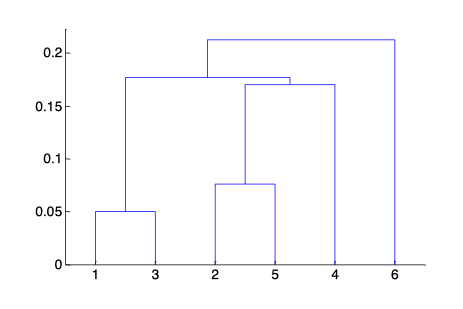
\includegraphics[width=\linewidth]{Dendrogramma.png}
  \caption{Dendrogramma nel clustering gerarchico}
\end{figure}

La cosa interessante è che a differenza di KMeans, in questo caso non dobbiamo specificare dei parametri come ad esempio il numero di cluster o i centroidi da cui far partire l'algoritmo.
Abbiamo due tipi di clustering gerarchico, quello agglomerativo in cui abbiamo un comportamento bottom-up (prima tanti cluster piccoli e poi unisco) e quello divisivo in cui abbiamo un comportamento top-down (prima un cluster unico poi divido).



\section{Funzionamento}

\begin{itemize}
    \item Ad ogni iterazione, presi tutti i punti, calcoliamo la matrice con le distanze;
    \item Prendiamo i punti a distanza minore tra loro e li uniamo in un unico cluster;
    \item Calcoliamo la distanza da quel cluster a tutti gli altri punti e prendiamo di nuovo la distanza minima creando un nuovo cluster;
    \item Una volta creato un cluster unico ci fermiamo.
\end{itemize}

\section{Calcolo della distanza: MIN}

Nel clustering gerarchico in versione MIN la prossimità di due cluster viene calcolata sulla base della distanza minima tra due punti di due differenti cluster.
La distanza minima (o single link) è in grado di gestire forme strane dei cluster ma ha problemi con gli outlier.
Nell'esempio di Figura 2 vengono prima uniti in un cluster 3 e 6 perchè sono a distanza minima l'uno dall'altro e poi 5 e 2.
Una volta che sono stati creati questi due cluster andiamo a considerare le distanze tra i punti in questi due cluster e gli altri punti esterni per capire quali unire.
Ad esempio tra i due cluster considero queste distanze e calcolo il minimo:
$min(dist(3,2), \ dist(6,2), \ dist(6,5), \ dist(3,5)$

\begin{figure}[H]
 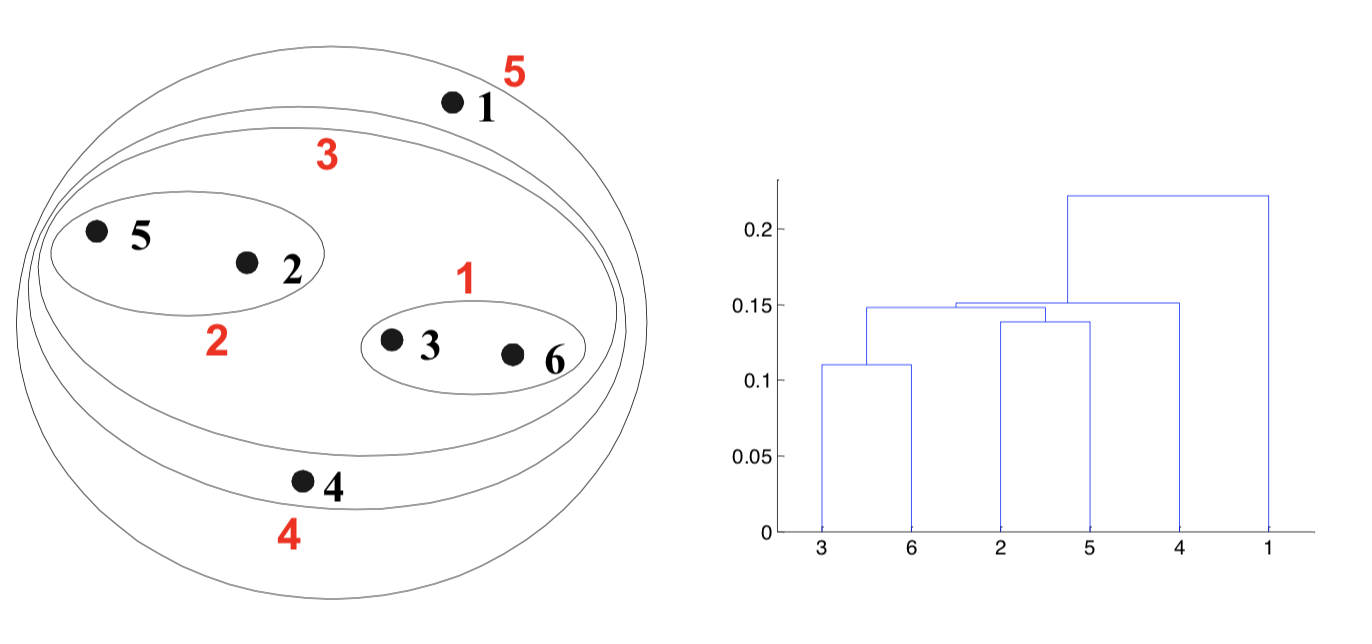
\includegraphics[width=\linewidth]{MIN.png}
  \caption{Clustering gerarchico con calcolo delle distanze con MIN}
\end{figure}

Poi devo considerare anche le distanze con gli altri punti. In ogni caso una volta fatti questi calcoli e presi i minimi nel caso delle distanze tra cluster e punti esterni devo aggiornare la matrice riducendo quindi le linee (perchè creo una sola riga per i cluster, ad esempio 3 e 6 diventano una sola riga della matrice).

\section{Calcolo della distanza: MAX}

Se uso la metrica MAX, vale più o meno il ragionamento fatto sopra, l'unica differenza riguarda il modo in calcolo la distanza tra i punti di un cluster e i punti esterni. Sopra usavo il minimo, qua uso il massimo:

$MAX(dist(3,2), \ dist(6,2), \ dist(6,5), \ dist(3,5)$


\begin{figure}[H]
  \centering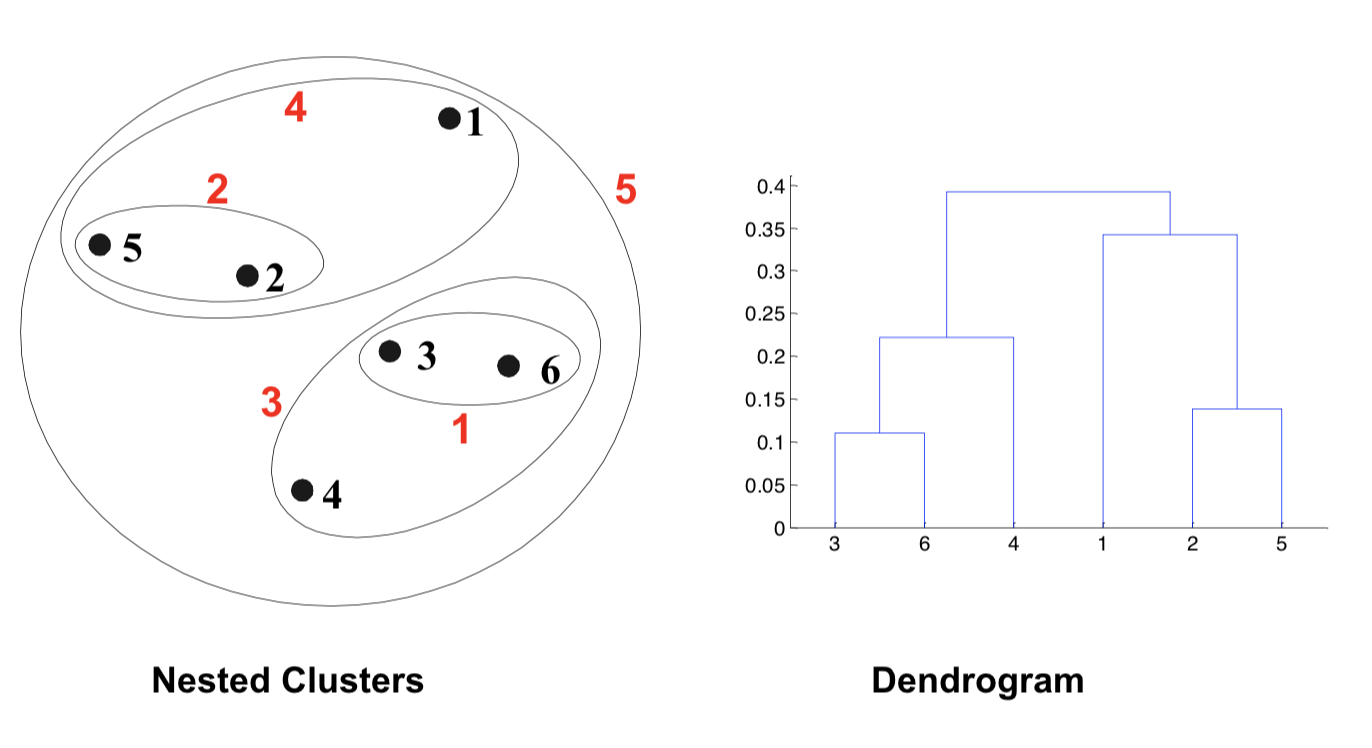
\includegraphics[width=\linewidth]{MAX.png}
  \caption{Clustering gerarchico con calcolo delle distanze con MAX}
\end{figure}

In questo caso MAX, che si chiama anche complete link, ha difficoltà a gestire cluster con forme particolari e divide i cluster che sono grandi. Gli outlier vengono uniti tardi perchè la distanza è maggiore rispetto ai punti normali, quindi nel dendrogramma verranno uniti alla fine.

{\bf Poi però una volta che ho aggiornato la matrice, va sempre e comunque presa la distanza MINIMA.}

\section{Calcolo della distanza: Group Average}

In questo caso la distanza tra i punti di un cluster e quelli esterni (o quelli di un secondo cluster) viene calcolata facendo la media di tutte le distanze.
Poi una volta aggiornata la matrice si prende la distanza minore.
In questo caso non abbiamo problemi con il rumore ma abbiamo problemi con cluster che hanno forme strane.

\section{Calcolo della distanza: Metodo dei centroidi}

In questo caso le distanze tra i cluster o tra un cluster si calcolano basandoci sul centroide del cluster.

\section{Calcolo della distanza: Metodo di Ward}

In questo caso consideriamo le possibili unioni di cluster distinti. Per ogni possibile unione calcoliamo la SSE dell'unione. Una volta calcolata l'SSE prendiamo l'unione che minimizza l'SSE.
Qui abbiamo problemi con cluster di forme strane ma non troppo con il rumore, il metodo Ward tende più a trovare cluster di forma circolare.

\section{Note}

Se usiamo la proximity matrix abbiamo bisogno di $O(n^2)$ spazio per memorizzare tutti i dati necessari.
Avendo n step allora avremo un costo di $O(n^3)$.

\subsection{Clustering Gerarchico Divisivo}

Oltre al cluster gerarchico agglomerativo, abbiamo anche un secondo tipo di clustering gerarchico che è chiamato Divisivo.
In questo caso partiamo da un cluster unico e poi dividiamo in cluster piccoli.
Per fare questo prendiamo i punti del piano e costruiamo il minimum spanning tree. Una volta costruito il grafo, prendiamo l'arco più lungo e lo spezziamo, creando due cluster. Andiamo avanti così fino a quando non abbiamo creato tutti cluster unici.

\chapter{DBSCAN}

DBScan è un algoritmo di clustering basato sulla densità dei punti.

Parametri:

\begin{itemize}
    \item Eps: raggio del cerchio che costruiamo intorno ad ogni punto
    \item MinPTS: numero minimo di punti che devono trovarsi all'interno del cerchio che creiamo attorno ai punti 
\end{itemize}

\section{Labellizzazione dei punti}

\begin{itemize}
    \item Un punto è considerato "Core Point" se all'interno del cerchio di raggio Eps che creiamo sono contenuti almeno MinPTS punti
    \item Un punto è "Border Point" se fa parte del cerchio di un core Point ma non ha attorno un numero di punti maggiore o uguale a MinPts
    \item Un punto è un "Noise Point" se non è Border e Core
\end{itemize}

\section{Creazione dei cluster}

Una volta labelizzati i punti vanno presi i core point. 
Creiamo un grafo in cui i core point che sono a distanza massima Eps sono collegati.
Alla fine ogni componente connessa del grafo rappresenta un cluster.
I punti Border invece vengono aggiunti al cluster più vicino, i Noise point invece non sono presi in considerazione.


\section{Note}

DBScan funziona bene in presenza di rumore e anche quando i cluster hanno forme strane. 
Non è in grado di riconoscere cluster con densità molto differenti tra loro.
Per determinare l'EPS dobbiamo calcolare la distanza di ogni punto del cluster dal suo K-esimo vicino più vicino.

\chapter{Cluster Validity}

Una volta eseguita una clusterizzazione, dobbiamo trovare un modo per valutarla e capire se è stato fatto un buon lavoro e se i pattern che abbiamo trovato sono dovuti al rumore. È utile anche perchè in questo modo riusciamo a fare un confronto tra i vari possibili algoritmi di clustering che possiamo utilizzare oppure per capire tra due set di cluster quale dei due è migliore.
Ci sono vari metodi per valutare una clusterizzazione, possiamo intanto distinguere tre tipologie:

\begin{itemize}
    \item Indici esterni: i cluster vengono valutati cercando di capire quanto la divisione in cluster rispecchia una classificazione dei vari dati che conosciamo a priori;
    \item Indici interni: cerchiamo di capire se i dati che sono presenti all'interno di ognuno dei cluster sono simili tra loro o no utilizzando solamente le informazioni che abbiamo a disposizione;
    \item Relative Index: Usato per confrontare due clusterizzazioni e capire quale delle due è migliore.
\end{itemize}



Possiamo utilizzare la correlazione per capire la qualità della clusterizzazione, in questo caso vengono create due matrici, una con le distanze tra i punti e una in cui inseriamo le somiglianze tra i punti (1 per ogni coppia di punti che stanno nello stesso cluster, 0 altrimenti). Studiando la correlazione capiamo se la clusterizzazioine è stata fatta bene o no.
Una correlazione alta tra le due matrici indica che i punti che appartengono allo stesso cluster sono veramente vicini tra di loro.

Se invece abbiamo due cluster e dobbiamo confrontarli per capire quale dei due è migliore, possiamo usare l'SSE. Lo calcoliamo in ognuno dei due cluster e poi confrontiamo cercando di capire quale dei due è minore.
La SSE potrebbe non funzionare bene se abbiamo cluster di forme strane.
Internamente ad una clusterizzazione possiamo calcolare:
\begin{itemize}
\item Cluster cohesion: SSE all'interno del cluster per capire se i punti sono vicini tra loro o se sono separati;
\begin{equation}
WSS = \sum_i \sum\limits_{x \in C_i} (x-m_i)^2
\end{equation}
Dove $m_i$ è il centroide del cluster.
\item Cluster separation: mi indica quanto sono separati i cluster tra di loro.
\begin{equation}
BSS = \sum_i |C_i| (m-m_i)^2
\end{equation}
Dove m è il punto medio tra i due cluster, $m_i$ è il centroide del cluster e $|C_i|$ è la dimensione del cluster i.
\end{itemize}

Altri metodi per giudicare una clusterizzazione:

\begin{itemize}
    
    \item Silhouette Coefficient: Calcoliamo per ogni punto nel cluster la distanza media dagli altri punti del cluster (A) e poi la distanza media dai punti degli altri cluster (B). Poi calcoliamo:
    \newline
     \begin{equation}
            S = \frac{(b-a)}{(max(a,b))}
    \end{equation}
    
    Dove S è il coefficiente di Silhouette. La silhouette deve essere alta (in questo modo riusciamo ad avere una buona cluster cohesion e una buona cluster separation) e vogliamo che sia un valore positivo, se è negativo vuol dire che la distanza media tra i punti dei vari cluster è minore della distanza media dei punti all'interno del cluster.
    La silhouette è un valore compreso tra -1 e 1.
    \item Entropia: se ho dati esterni che indicano le etichette dei punti e ho calcolato i cluster posso usare l'entropia per dare un giudizio sulla qualità del cluster. L'entropia infatti mi indica quanto gli oggetti che finiscono nello stesso cluster sono davvero appartenenti alla stessa classe.
\end{itemize}

\section{Determinare il numero corretto di cluster}

Per capire quanti cluster devono essere creati è possibile calcolare l'SSE e la silhouette al variare del numero dei cluster che vogliamo ottenere.
Questo ci permette di avere due grafici, uno per l'SSE e uno per la Silhouette.

\begin{figure}[H]
\centering
  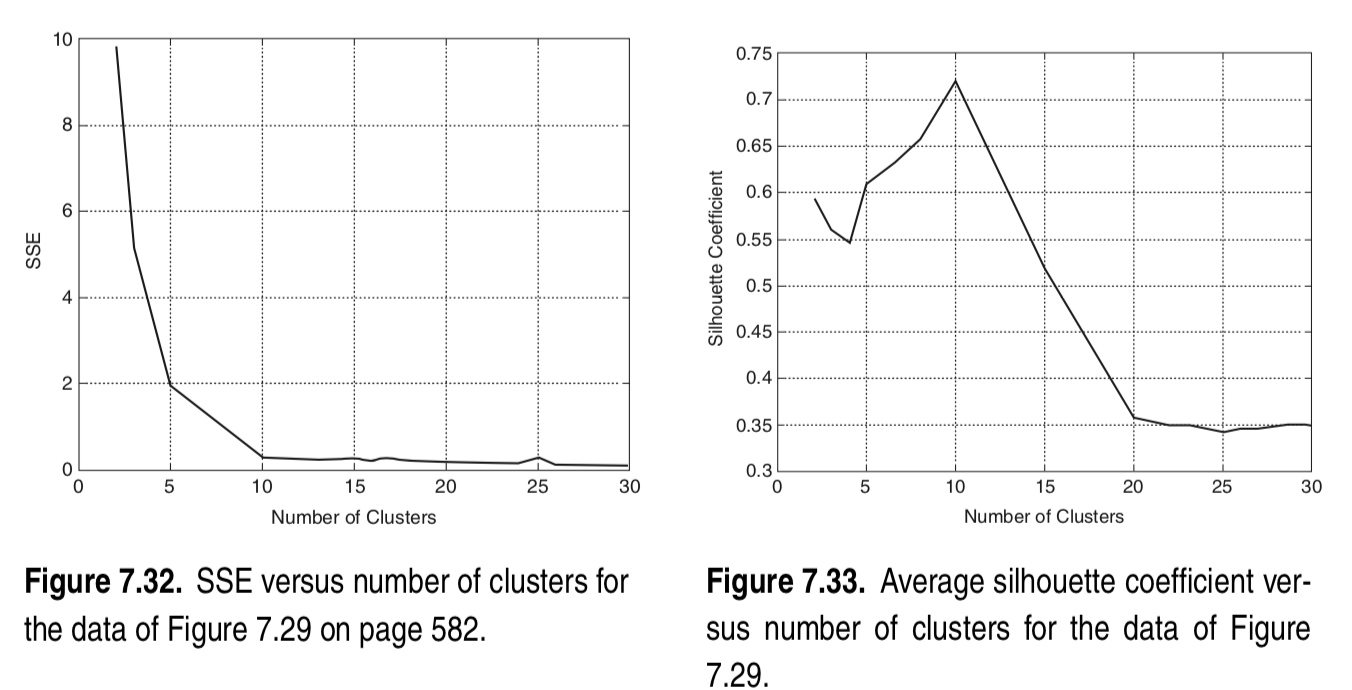
\includegraphics[width=\linewidth]{Knee.png}
\end{figure}

In quello dell'SSE cerchiamo il punto di gomito mentre in quello della silhouette cerchiamo il picco più alto. Il punto in corrispodenza di queste due forme particolari del grafico è quello che mi indica quanti cluster voglio creare.

\chapter{Classificazione}
Con classificazione si intende il procedimento che, partendo da un insieme di dati chiamato training set, in cui i vari record sono nel formato $<X, Y>$ dove X sono gli attributi e Y la classe di appartenenza di quel record, cerca di predire la classe di appartenenza dei record che non sono stati ancora analizzati.
Quello che si fa in questo procedimento è andare a creare un modello che mappi ognuno degli attributi X in una classe, il test di questo modello poi viene effettuato su un insieme di dati chiamato Test Set. L'accuratezza del modello viene determinata utilizzando il Test Set.
Un problema di questo tipo è detto supervisionato perchè per creare il modello abbiamo a disposizione un insieme di dati che sono già classificati. 
Quando il modello classifica i record del dataset solamente in base alle classi abbiamo una classificazione mentre invece se dobbiamo predire attributi numerici, questo procedimento si chiama regressione.

Ci sono vari modi per svolgere la classificazione, uno di questo è il Decision Tree.
La creazione di un decision Tree prevede vari passaggi, il primo è la comprensione dell'algoritmo di induzione del decision tree, poi dobbiamo creare il modello e successivamente applicarlo ai nuovi dati.

Per la fase di induzione che ci porta alla creazione del modello abbiamo vari algoritmi, uno di questi è l'algoritmo di Hunt.
Funzionamento dell'algoritmo di Hunt:
\begin{itemize}
    \item Abbiamo un dataset segnato in cui ogni record è segnato con una certa classe (ad esempio Si o No). Partiamo da un nodo unico in cui segnamo il numero di record Si e il numero di record No.
    \begin{figure}[h!]
  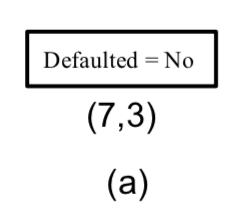
\includegraphics[width=0.3\linewidth]{Hunt1.png}
  \caption{Algoritmo di Hunt}
\end{figure}
    \item Se tutti i record appartengono alla stessa classe ci fermiamo, altrimenti scegliamo un attributo e lo mettiamo in un nodo, poi dividiamo i figli di quell'attributo in base ai possibili valori dell'attributo e gli associamo come figli le classi associate nel dataset.
    \begin{figure}[h!]
  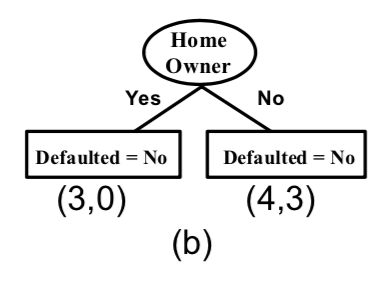
\includegraphics[width=0.3\linewidth]{Hunt2.png}
  \caption{Algoritmo di Hunt}
\end{figure}
    \item Ricorsivamente andiamo ad eseguire lo stesso procedimento, se le classi sono separate e quindi abbiamo ad esempio che nella foglia 3 record sono Si e 0 no allora ci fermiamo, altrimenti prendiamo un altro attributo e lo espandiamo ancora.
    \begin{figure}[h!]
  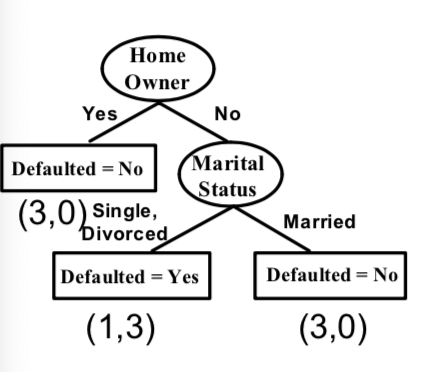
\includegraphics[width=0.3\linewidth]{Hunt3.png}
  \caption{Algoritmo di Hunt}
\end{figure}
\end{itemize}

\section{Condizione di test di un attributo}

Dato un nodo che contiene un attributo abbiamo vari modi per splittarlo e creare dei figli o delle foglie:

\begin{itemize}
    \item Per gli attributi nominali (tipo sposato, single, vedovo) abbiamo la possibilità di fare uno split Binario, in questo caso dobbiamo riunire gli attributi in due set e dividere in due rami il nodo. Alternativamente possiamo avere uno split multi way e quindi dividiamo l'attributo in tanti rami quanti sono i valori possibili per quell'attributo.
    \item Attributi ordinali (tipo piccolo, medio, grande): in questo caso dobbiamo fare o uno split multi way oppure possiamo anche farlo binario stando però attenti a mantenere l'ordine degli attributi nel momento in cui li dividiamo in due set.
    \item Per gli attributi continui (tipo 80K) possiamo fare una divisione binaria dividendo in base al minore di o maggiore di. Possiamo estendere questa divisione ad una divisione multi way andando a dividere in base a bucket più piccoli (tipo minore di 20, minore di 50 e maggiore di 20 ecc).
\end{itemize}

\subsection{Come determinare il miglior split}

Se prendo un nodo singolo e devo dare una valutazione per capire il valore della sua impurità posso utilizzare tre misurazioni differenti:

\begin{itemize}
    \item La prima misurazione possibile è l'entropia:
        \begin{equation}
            Entropy = - \sum\limits_{i=0}^{c-1} p_i(t)* \ log_2\ p_i(t)
        \end{equation}
        
    In questo caso $p_i(t)$ è la frequenza delle istanze di training appartenenti ad una certa classe rispetto al numero totale di record e c è il numero delle classi.
    L'entropia ha valore minimo pari a 0 e massimo pari a 1. Quando è 0 vuol dire che i dati sono divisi molto bene. Quindi ad esempio se abbiamo due classi possibili (SI e NO) con 1 NO e 5 SI, l'entropia si calcola come \newline
    \begin{equation}
            Entropy = - (1/6) \ log_2 \ (1/6) - (5/6) \ log_2 \ (5/6)
    \end{equation}
    
    \item Un'altra possibile misurazione è il Misclassification Error:
    \begin{equation}
        MisError = 1 - max(P((i|t))
    \end{equation}
    Dove $max(P((i|t))$ è il valore massimo che abbiamo con lo split dei dati, ad esempio se ho 6 record, 5 vengono classificati come SI e uno come NO allora abbiamo che $5/6$ è il $max(P((i|t))$ perchè $5/6 > 1/6$.

    \item Poi c'è il Gini Index:
        \begin{equation}
            Gini \ Index = 1 - \sum\limits_{i=0}^{c-1} p_i(t)^2
        \end{equation}
    Dove $P_i(t)$ viene calcolato come con l'entropia, se ad esempio abbiamo una classe Si che ha associati 3 record e una no che ne ha associati 4 allora P(C1) sarà $\frac{3}{7}$ e P(C2) sarà $\frac{4}{7}$.
    Poi nel calcolo del Gini questi risultati vanno elevati al quadrato.
    Quindi ad esempio se abbiamo due classi possibil (SI e NO) con 1 NO e 5 SI, il Gini Index si calcola come \newline
    \begin{equation}
            Gini = 1 - (1/6)^2 - (5/6)^2
    \end{equation}
    
    Possiamo calcolare il Gini Index anche su una serie di nodi.
    
    \begin{equation}
    Gini \ Index = \sum\limits_{i=0}^{c-1} \frac{n_i}{n} * Gini(i)
    \end{equation} 
        
    Se ad esempio abbiamo un albero come:
    
    \begin{figure}[h!]
    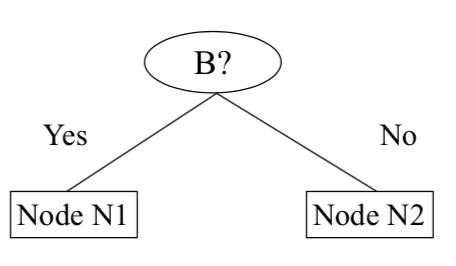
\includegraphics[width=0.3\linewidth]{Gini1.png}
    \caption{Esempio Gini Index}
    \end{figure}
    Allora vediamo prima che la divisione delle classi per il nodo B è 7 Si e 5 No. Poi splittando abbiamo che nel nodo n1 diventa 5 si e una no, nel nodo 2 diventa 2 si e una no. 
    Quindi calcoliamo il Gini di N1 e il Gini di N2 e poi il Gini pesato su tutti i nodi. Quindi per il calcolo del gini pesato consideriamo il numero complessivo di record e il numero dei record di N1 e N2.
    Quindi sarebbe
        \begin{equation} 
            Gini Pesato = \frac{6}{12} * Gini(N1) + \frac{6}{12} * Gini(N2)
    \end{equation}
    
    
    \item Poi c'è l'errore di classificazione (Misclassification Error):
        \begin{equation}
            Errore\ di\ classificazione = 1 - max_i[p_i(t)]
        \end{equation} 
    Quindi ad esempio se abbiamo due classi possibil (SI e NO) con 1 NO e 5 SI, il Gini Index si calcola come \newline
    \begin{equation}
            Errore\ di\ classificazione = 1 - max[(1/6),(5/6)]
    \end{equation}
    \end{itemize}
    
\subsection{Valutazione di tutti i nodi figli}

Se ho un certo nodo che ha N istanze di training e poi ha k figli $v_1, ... , v_k$ con $N(v_j)$ che è il numero di istanze di training del figlio $v_j$ allora possiamo calcolare l'impurità complessiva dei figli come:

\begin{equation}
    I(children) = \sum\limits_{j=1}^{k} \frac{N(v_j)}{N} I(v_j)
\end{equation}

In questo caso per ognuno dei K figli calcoliamo l'impurità del nodo e poi la moltiplichiamo per il numero delle istanze di quel figlio diviso per il numero di istanze complessive.

Un esempio usando l'entropia per calcolare l'inpurità dei nodi figli:


\begin{figure}[H]
  \centering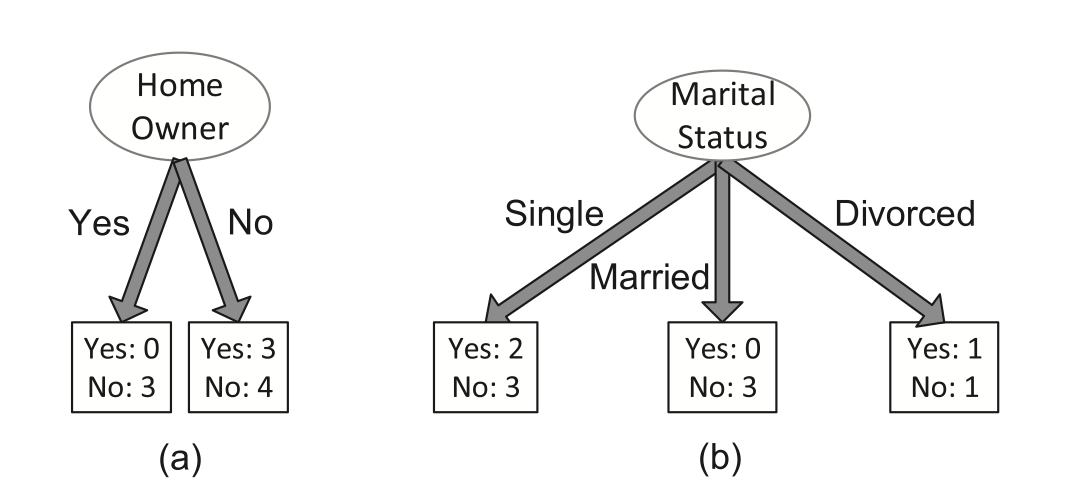
\includegraphics[width=\linewidth]{TestCondition1.png}
  \caption{Alberi che possiamo creare prendendo due attributi diversi, Home Owner e Marital Status}
\end{figure}
\newline\newline$I(Home\ Owner = Yes) = - (0/3)\ log_2\ (0/3)\ -\ (3/3)\ log_2\ (3/3) = 0$
\newline
$I(Home\ Owner = No) =  - (3/7)\ log_2\ (3/7)\ -\ (4/7)\ log_2\ (4/7) = 0.985 $ \newline
$I(Children) = I(Home\ Owner) = (3/10) * 0 + (7/10) * 0.985 = 0.690
$  \newline\newline$I(Marital \ Status = Single) =- (2/5)\ log_2\ (2/5)\ -\ (3/5)\ log_2\ (3/5) = 0.971$  \newline
    $I(Marital \ Status = Married) = - (0/3)\ log_2\ (0/3)\ -\ (3/3)\ log_2\ (3/3) = 0$ \newline
    $I(Marital \ Status = Divorced) = - (1/2)\ log_2\ (1/2)\ -\ (1/2)\ log_2\ (1/2) = 1$ \newline
    $I(Children) = I(Marital \ Status) = (5/10) * 0.971 + (3/10) * 0 + (2/10) * 1 = 0.686$
\newline
\newline
Quindi tra i due l'attributo Marital Status ha una entropia pesata minore, quindi sarebbe da preferire.

    
\subsection{Come identificare il miglior attributo da usare come condizione di test}

Per capire quale attributo scegliere si deve andare a calcolare il \b{gain}. Ovvero:
\begin{equation}
    \Delta = Gain = I(Parent) - I(Children)
\end{equation}

Il calcolo di I(Children) è spiegato nel paragrafo precedente. 
Il calcolo di I(Parent) ci permette di capire l'inpurità che ha il padre prima di scegliere un nuovo attributo da usare come test condition. Quindi se devo provare più di una test condition questo valore non cambia e l'unica cosa che va calcolata ogni volta è I(Children).

I(Parent) viene calcolato considerando l'entropia (O il Gini Index o il Miscassification Error) sul nodo padre, andando quindi a dividere e a contare le istanze che portano ad una certa classe da quelle che portano ad un'altra classe.
Se consideriamo l'entropia come misurazione sia per il padre che per il figlio allora il gain si chiama "Information Gain".
Questo (Information) gain serve per capire la riduzione dell'entropia dovuta allo split, alla fine verrà scelto lo split che massimizza il gain.

Un esempio, prendiamo la Figura 4 e consideriamo I(Parent):

\begin{equation}  
    I(Parent) = - (3/10)\ log_2\ (3/10) - (7/10)\ log_2\ (7/10) = 0.881
\end{equation}

Poi possiamo calcolare il gain andando a calcolare:
\begin{equation}
    \Delta = Gain = I(Parent) - I(Children)
\end{equation}
Alla fine scegliamo l'attributo che produce il gain più alto.
Ovvero, nel caso della scelta di Home Owner come attributo calcoliamo:

\begin{equation}
    \Delta = Gain = 0.881 - 0.690 = 0.191
\end{equation}

Nel caso di Marital Status calcoliamo:


\begin{equation}
    \Delta = Gain = 0.881 - 0.686 = 0.195
\end{equation}

Quindi tra i due dovremmo scegliere l'attributo Marital Status.

Sia per I(Parent) che per I(Children) possiamo utilizzare una delle metriche indicate in precedenza (entropia, gini index).

\subsection{Gain Ratio}

Nel paragrafo precedente abbiamo detto che preferiamo l'attributo Marital Status perchè il gain è minore rispetto all'Home Owner.
Il problema delle misurazioni viste (Gain, Entropia, Gini Index) è che tendono a prediligere quegli attributi che splittano le istanze in più figli. Quindi se avessimo un attributo ID che è diverso per ogni istanza, l'information gain ci direbbe di utilizzare questo anche se non ci dice niente dal punto di vista della classificazione.
Quindi è stata introdotta una misurazione chiamata Gain Ratio che invece tiene in considerazione il numero di figli che si creano partendo dalla scelta di un attributo e tende a penalizzare i partizionamenti che creano un gran numero di partizioni.
Il gain Ratio si calcola in questo modo:

\begin{equation}
    Gain\ Ratio = \frac{\Delta_{info}}{Split\ Info} = \frac{Entropy(Parent) - \sum\limits_{j=1}^{k} \frac {N(v_i)}{N} Entropy(v_i)}{- \sum\limits_{i=1}^{k} \frac{N(v_i)}{N} log_2 \frac {N(v_i)}{N}}
\end{equation}

Dove N è il numero totale di istanze, $N(v_i)$ è il numero di istanze per quel nodo specifico. K invece è il numero totale di split.

\begin{figure}[h!]
  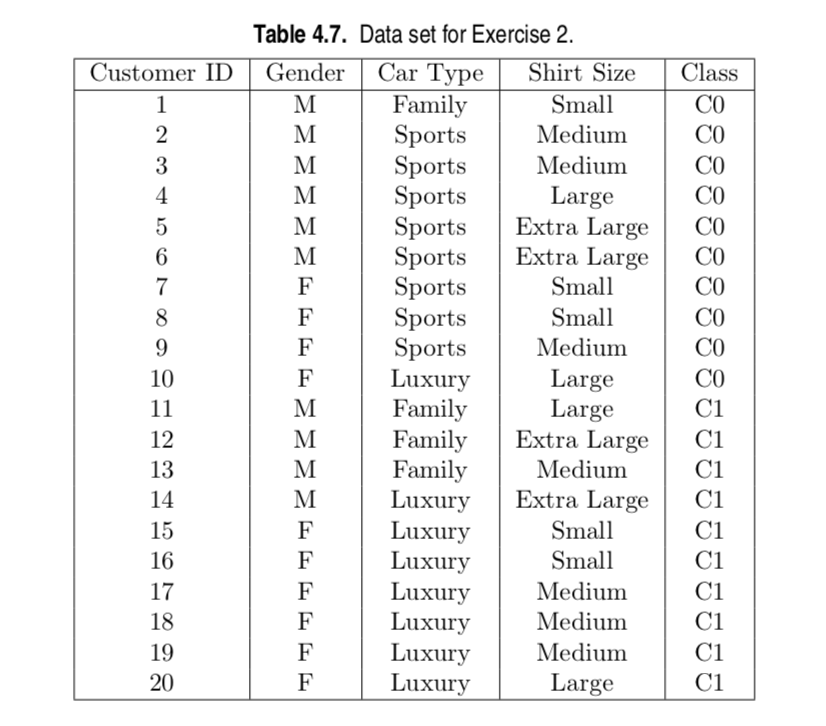
\includegraphics[width=\linewidth]{DatasetMacchine.png}
  \caption{Dataset di esempio}
\end{figure}

Un esempio con il dataset della Figura 5.

\begin{itemize}
    \item Dobbiamo selezionare il miglior attributo tra Gender, Car Type e Customer ID. Quindi vogliamo usare la formula del gain ratio. Calcoliamo Entropy(Parent).
    \newline
    \begin{equation}
        Entropy(Parent) = - (10/20) log_2(10/20) - (10/20) log_2(10/20) = 1
    \end{equation} 
    \item Poi devo calcolare l'entropia dei vari figli, con Gender avremmo:
    \newline
    $Entropy(Gender) = (10/20)\ *\ Entropy(Gender = M)\ +\ (10/20)\newline * Entropy(Gender = F)\ = \ (10/20)\ * \ (-(6/10)\ log_2\ (6/10)) +\ (10/20)\ *\ (-(4/10)\ log_2\ (4/10)) = 0.971$ 

    Per Car Type:
    
    $Entropy(Car Type) = (8/20)\ *\ Entropy(CarType = Sport)\ +\ (4/20)\newline * Entropy(CarType = Family)\ +\ (8/20) * Entropy(CarType = Luxury)   \newline = \ (8/20)\ * \ (-(8/8)\ log_2\ (8/8)) +\ (4/20)\ *\ (-(1/4)\ log_2\ (1/4) -(3/4)\ log_2\ (3/4)) +\ (8/20)\ *\ (-(1/8)\ log_2\ (1/8) -(7/8)\ log_2\ (7/8) ) = 0.380$ 
    
    Per Customer ID:
    
    $Entropy(Customer ID) = (1/20)[-(1/1) log_2 (1/1) - (0/1) log_2 (0/1)] * 20 = 0$
    
    \item Ora calcoliamo anche il Gain Ratio per tutti e tre gli attributi:
    
    $Gain Ratio(Gender) = \frac{1 - 0.971}{-(10/20) log_2 (10/20) - (10/20) log_2 (10/20)} = 0.029$
    
    $Gain Ratio(Car Type) = \frac{1 - 0.380}{-(8/20) log_2 (8/20) - (4/20) log_2 (4/20) - (8/20) log_2 (8/20)} = 0.41$
    
    $Gain Ratio(CustomerID) = \frac{1 - 0}{-(1/20) log_2 (1/20) * 20} = 0.23$
\end{itemize}

In questo caso usando il solo Information Gain avremmo preferito l'attributo Customer ID perchè ha tanti figli e quindi divide bene le classi. Andando però a calcolare il Gain Ratio, questo attributo ha un valore più basso rispetto ad esempio a Car Type e quindi scegliamo Car Type.

\section{Caratteristiche dei decision Tree}

\begin{itemize}
    \item I decision tree possono essere applicati a qualsiasi dataset senza avere la necessità di fare modifiche sui dati e senza dover considerare la probabilità della distribuzione delle varie classi e degli attributi.
    \item È un sistema efficiente perchè, dato che possiamo creare una grande quantità di alberi di decisione, vengono utilizzati degli algoritmi greedy per fermarsi prima di generare alberi troppo complicati.
    \item I decision Tree funzionano anche con i Missing Values.  Se sono presenti nel test set allora utilizza un metodo probabilistico per splittare comunque il nodo e andare in un certo percorso dell'albero.
    \item Un decision Tree può gestire la presenza di attributi ridondanti, come ad esempio gli attributi che sono molto correlati tra loro. Ci possiamo accorgere di attributi ridondanti quando vediamo che il gain tra la scelta di due attributi non è poi così distante.
    \item L'albero di decisione è in grado di gestire anche gli attributi irrilevanti, un attributo è irrilevante se non è utile per la classificazione e quindi la sua presenza va solamente a rendere più complesso l'albero senza portare un miglioramento in termini di performance.
    \item La complessità della costruzione del decision tree è la seguente: $O(M*N*Log N)$ dove N è il numero di record, M è il numero di attributi.
 
\end{itemize}

Abbiamo anche degli svantaggi per quanto riguarda l'utilizzo dei decision tree.
Una minima modifica all'interno del dataset può comportare grandi cambiamenti all'interno del decision tree.
Il decision tree che otteniamo può diventare eccessivamente complicato.
In alcuni casi il singolo decision tree non è in grado di fare previsioni accurate e quindi si dovrebbe preferire l'utilizzo di un random forest (metodo ensemble learning in cui usiamo tanti decision tree costruiti con subset di dati presi dal dataset iniziale e poi classifichiamo il record con ognuno di questi classificatori. Alla fine si prende la moda delle classificazioni ottenute).

L'albero di decisione non è in grado di gestire l'interazione tra gli attributi. Si parla di interazione tra gli attributi quando vogliamo indicare che un attributo preso singolarmente non è in grado di darci troppe informazioni mentre se lo prendiamo in coppia con altri attributi può permetterci di predire meglio.
    Nei classici decision tree in ogni nodo scegliamo un attributo e alla fine ci fermiamo quando la scelta di un attributo ci porta ad una divisione precisa delle classi (tipo tutti record di un tipo e 0 o pochi di un altro).
    Quindi con questo decision tree andiamo a creare una immaginaria divisione all'interno di un piano tra i vari record sulla base degli attributi scelti.
    Questo bordo che divide i vari attributi è chiamato decision boundary, se scelgo un solo attributo alla volta per splittare, il decision boundary sarà sempre una retta perpendicolare all'asse delle X o delle Y.
    Se invece di testare un attributo alla volta volessi usare all'interno di un nodo più di un attributo, ci troveremmo nella situazione in cui avremmo un decision boundary differente in cui la retta che divide diventa obliqua (usando due attributi).

Come già detto il numero di possibili alberi di decisione è molto grande e poi ogni scelta all'interno dell'albero riguarda un solo attributo alla volta.
Un altro problema è legato al fatto che a mano a mano che scendiamo all'interno dell'albero, il numero delle istanze diminuiscono e in particolare nelle foglie questo numero potrebbe essere così basso da non rappresentare un valore adeguato per fare una statistica.

\section{Problemi della classificazione: Underfitting e Overfitting}

Quando lavoriamo con l'albero di decisione abbiamo un dataset diviso in questo modo:
\begin{itemize}
    \item Training set: parte del dataset su cui fare il training. Il training set lo usiamo per produrre il modello. Il modello testato su questo dataset produce un errore di training.
    \item Validation Set: parte del dataset (comunque con i record segnati) su cui testiamo il modello. Un modello testato su questo dataset produce un errore di validazione. Questo set di dati viene utilizzato per fare il tuning degli iperparametri.
    \item Test Set: è il dataset su cui effettivamente testare il modello, produce l'errore di generalizzazione.
\end{itemize}

Quando creiamo un albero di decisione possiamo avere due problemi principali:

\begin{itemize}
    \item Il modello che abbiamo sviluppato è troppo semplice, quindi l'errore che otteniamo sul training set e sul test set è troppo elevato. In questo caso si parla di underfitting.
    Questo problema si verifica, ad esempio, se utilizziamo pochi attributi.
    \item Un problema opposto è l'overfitting, questo si verifica quando abbiamo un modello eccessivamente complesso, quindi ad esempio un albero con troppi nodi. In questo caso il modello è troppo legato ai dati di training, su cui produce un errore basso, ma non predice bene su dati che non ha ancora visto, quindi l'errore di test e di generalizzazione sarà molto alto.
    L'overfitting può essere causato anche dalla presenza di pochi dati di training, in questo caso il modello sarà infatti trainato su questi pochi dati ma non sarà in grado di generalizzare. Un altro motivo che porta all'overfitting è la presenza dei noise point.
\end{itemize}

\section{Model Selection}

Con Model Selection intendiamo il processo di scelta di un modello rispetto ad un altro basato sull'errore di generalizzazione del modello (vogliamo quello che ha l'errore di generalizzazione più basso).

Presi i dati che abbiamo a disposizione per creare il modello si deve per prima cosa dividere il training set in due porzioni, questo primo metodo si chiama Holdout. Una prima porzione ($2/3$ del totale, chiamata development set) è quella che utilizziamo per il training del modello mentre la seconda ($1/3$ del totale) la utilizziamo per il test del modello (model evaluation) ovvero per calcolare quando il modello è in grado di predire.
Quindi prima facciamo il training del modello e poi andiamo a provarlo sui dati di test.
Alla fine scegliamo quel modello che ha l'errore più basso sul dataset di test.

Il development set viene poi diviso in training set e validation set. Sul training set facciamo il train del modello e creiamo vari modelli con parametri differenti tra loro, poi sul validation set possiamo provare il modello e se ne abbiamo vari con parametri differenti sceglieremo il modello predice meglio.
Alla fine, scelti i parametri che mi permettono di avere una migliore predizione sui dati validation possiamo fare nuovamente il training del modello su tutto il development set.
Un’altra soluzione che possiamo utilizzare quando abbiamo pochi dati a disposizione per fare il training è il KFold Cross validation. In questo caso dividiamo prima in training set e test set, poi il training set viene diviso in K set. Di questi K set ogni volta ne teniamo alcuni per fare la validation del modello e alcuni per fare il training del modello.
C’è da pensare questo procedimento come due for innestati: un primo for esterno fissa gli iperparametri (ne proviamo vari) poi un secondo for interno invece fa il training del modello su parte dei K set di dati e fa la validation sui set rimanenti. Poi per ognuno dei parametri facciamo la media dell’errore che abbiamo ottenuto facendo il test sul set validation.

Una evoluzione del primo modello consiste nell'utilizzare il Model Selection in coppia con la Model Complexity. Questo vuol dire che per la scelta del modello non utilizzo solamente una funzione che mi indica la quantità dell'errore sul validation set ma utilizzo anche la complessità del modello.
In questo caso si utilizza il principio di Occam's che dice che se ho due modello che producono lo stesso errore, dovrò preferire quello che è meno complesso.
Per questo motivo la scelta del modello viene effettuata basandosi su questa formula:
\begin{equation}
    Generalization\ Error = train.error(m, D.train) + \alpha * complexity(m)
\end{equation}

Dove m è il modello che abbiamo prodotto e D.train è il dataset di training. La $\alpha$ viene utilizzata come parametro per indicare quanto è importante la complessità del modello rispetto all'errore di training.

La complessità nominata all'interno della formula e relativa ad un albero di decisione può essere calcolata in vari modi.
Un primo metodo considera la dimensione del dataset di training e il numero di foglie che ho creato all'interno dell'albero.
In particolare se il mio albero di decisione ha K foglie e N istanze di training allora: $Complessità(T) = \frac{K}{N}$.

Un altro metodo che mi permette di calcolare la complessità dell'albero di decisione consiste nell'utilizzo del "Minimum Description Length" detto anche MDL.
In questo caso abbiamo un dataset labellato e costruiamo un albero di decisione partendo da questo dataset. Ora, se vogliamo indicare ad un'altra persona come utilizzare il nostro modello per fare previsioni sul dataset che noi abbiamo usato come training possiamo o passargli il dataset labellato oppure passargli l'albero di decisione prodotto.
Se l'albero di decisione funziona bene inviamo solamente l'albero, altrimenti dobbiamo segnare anche i record che l'albero non riconosce correttamente.
In questo secondo caso non inviamo solamente i bit del modello ma anche dei bit aggiuntivi per segnalare che alcune previsioni non sono corrette.
Quindi la complessità del modello è data da:
\newline
$Cost(model,data) = Costo\ invio\ istanze\ non\ classificate\ + \alpha \ *\ Costo\ modello$

\section{Come evitare l'overfitting}

L'overfitting è quella situazione in cui possiamo trovarci quando creiamo un modello e si verifica uno dei due casi:
\begin{itemize}
\item Abbiamo pochi dati di training e quindi non generalizziamo bene su dati che non abbiamo mai visto
\item Il modello è troppo legato ai dati del training set dove abbiamo un errore basso poi sul test set l'errore è alto. il modello in questo caso sarà troppo complicato.
\end{itemize}

Il contrario dell'overfitting è l'underfitting in cui invece il modello è troppo semplice e abbiamo un erorre di training e di test che sono troppo alti.

Per evitare che il nostro modello vada in overfitting abbiamo due strategie possibili quando si utilizza un albero di decisione:

\begin{itemize}
    \item Pre-Pruning: In questo caso partendo dal dataset iniziamo a costruire l'albero di decisione, ad ogni nodo che espandiamo andiamo a calcolare il gain. Se il gain scende sotto ad un certo valore possiamo fermarci e non continuare l'espansione.
    Il vantaggio in questo caso è che non produco degli alberi troppo grandi, lo svantaggio è che potrei fermarmi troppo presto e in questo caso andrei a non considerare dei rami che invece potrebbero essere interessanti.
    \item Post-Pruning: in questo caso espandiamo tutto l'albero di decisione e poi, partendo dalle foglie andiamo a calcolare il gain cercando di capire quali possono essere eliminate.
    Il post pruning tende a restituire dei risultati che sono migliori rispetto a quelli che vengono restituiti dalla creazione dell'albero con il pre-pruning.
\end{itemize}

\section{Valutazione di un modello}

Una volta svolta la model selection in cui abbiamo considerato l'errore sui dati di training.Test, va effettuata la fase di model evaluation in cui andiamo a valutare il modello scelto basandoci però sui dati di test.
Durante questa fase possiamo effettuare per prima cosa una analisi delle performance del modello. 
Creiamo quindi una confusion Matrix ovvero una matrice 2x2 in cui inseriamo il numero dei record labellati come Si che sono stati classificati come Si ovvero i true positive (TP), poi quelli che sono No e No ovvero i true negative (TN) e poi falsi positivi FP e falsi negativi FN.
Una volta compilata la tabella possiamo andare a calcolare la valutazione dell'accuracy di questo modello:
Accuracy = $\frac{TP+TN}{TP+TN+FP+FN}$

Sempre sulla stessa matrice 2x2 possiamo andare a calcolare anche una misurazione differente relativa al costo della classificazione, partendo da questa matrice possiamo calcolare:
\newline
Precision = $\frac{True\ Positive}{Actual\ Results}$ = $\frac{TP}{TP+FP}$
\newline
Recall = $\frac{True\ Positive}{Predicted\ Results}$ = $\frac{TP}{TP+FN}$
\newline 
F-Measure = $2*\frac{Precision*Recall}{Precision+Recall}$ = $\frac{2TP}{2TP+FN+FP}$

In particolare:
\begin{itemize}
\item La precision indica la capacità del modello di trovare risultati rilevanti, mi dice la parcentuale dei risultati che sono rilevanti per il mio modello e che sono effettivamente rilevanti. 
Mi dice quanti sono quelli che ho classificato come positivi e che lo sono davvero rispetto al totale di quelli che ho sono positivi.
Un esempio può essere la classificazione di un terrorista,\newline $\frac{Record\ classificati\ come\ terroristi}{Record\ classificati\ come\ terroristi\ +\ record \ terroristi\ ma\ che\ in\ realtà\ non\ lo\ sono}$.
Qua se io classifico tutti come terroristi ho una precision pessima perchè ho un alto valore di False positive.
\item La recall indica la percentuale dei risultati rilevanti classificati correttamente dall'algoritmo. Mi dice quanti sono quelli che ho classificato come positivi rispetto (True positivi) a quelli che sono davvero positivi (true positive più falsi negativi). Ad esempio se devo classificare una persona in un modo o in un altro magari mi interessa massimizzare la recall perchè mi dice quante volte classifico bene quella persona rispetto alle volte che la classifico bene più le volte che la classifico male (falso negativo).
Un esempio può essere la classificazione di un terrorista,\newline $\frac{Record\ classificati\ come\ terroristi}{Record\ classificati\ come\ terroristi\ +\ record \ terroristi\ ma\ classificati\ come\ NON\ terroristi}$.
Qua se io classifico tutti come non terroristi ho una recall pessima perchè ho un alto valore di False negative.
\item L'F1 score è la media armonica di precision e recall.
\end{itemize}

Non possiamo massimizzare contemporaneamente sia la precision che la recall, quindi abbiamo l'F1 score. Se precision e recall sono entrambi importanti possiamo selezionare il modello che massimizza l'F1 score, negli altri casi si usa un tradeoff.



Oltre alla confusion matrix è anche possibile creare una cost matrix. In questa seconda matrice inseriamo il costo che vogliamo assegnare ad ognuna delle predizioni e poi calcoliamo il costo che otteniamo considerando le previsioni corrette e quelle errate.


\section{Model Comparison}
In questa fase abbiamo dei modelli "concorrenti" e vogliamo trovare un modo per dare un giudizio sulle performance di questi modelli.
Per la fase di model comparison possono essere utilizzate le curve Roc che ci permettono di confrontare due modelli.
La curva roc è una curva di probabilità che mi indica quanto il modello è capace di distinguere tra le classi, in particolare la curva roc è in grado di dirmi quanto il numero degli esempi che vengono classificati correttamente varia in base al numero degli esempi che vengono classificati negativamente.
Sull'asse X della curva roc abbiamo il false positive rate (FPR) e sull'asse Y abbiamo il true positive rate (TPR).
Questi due valori vengono calcolati in questo modo:
\begin{equation}
TPR = \frac{TP}{TP+FN}
\end{equation}

\begin{equation}
FPR = \frac{FP}{FP+TN}
\end{equation}

Come costruisco la curva:
\begin{itemize}
\item Per ognuna delle istanze di test devo calcolare la probabilità che la classe predetta sia quella positiva data P(+|A).
\item Ordino le istanze in ordine di probabilità crescente
\item Applichiamo un threshold
\item Contiamo il numero di FP, TN, FN e TP.
\item Calcoliamo il TPR e il FPR per ognuno dei punti e poi rappresentiamo il punto nel piano.
\end{itemize}

Ora la curva roc sarà differente a seconda di come il modello è in grado di classificare:
\begin{itemize}
\item Nella situazione ideale il modello classifica perfettamente e quindi abbiamo una divisione netta tra i positivi e i negativi. La curva quindi è perpendicolare sull'asse Y e poi parallela all'asse X. Se le curve non si sovrappongono il modello distingue perfettamente le classi negative dalle classi positive.
\begin{figure}[H]
\centering
  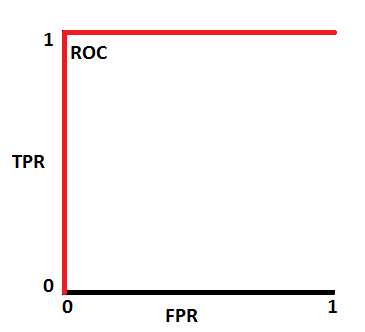
\includegraphics[width=0.3\linewidth]{optimal.png}
\end{figure}
\item Nella situazione più normale abbiamo un overlap quindi ci sono delle situazioni in cui il modello non mi classifica perfettamente.
\begin{figure}[H]
\centering
  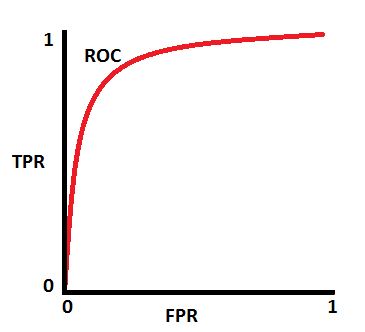
\includegraphics[width=0.3\linewidth]{good.png}

\end{figure}
\item Abbiamo poi una situazione che non va bene che è quella in cui X=Y e quindi ci troviamo con un modello che non sa scegliere
\begin{figure}[H]
\centering
  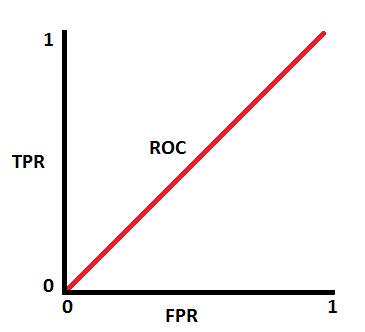
\includegraphics[width=0.3\linewidth]{bad.png}

\end{figure}
\item La situazione peggiore è quella in cui il modello sceglie il contrario di quello che dovrebbe scegliere.
\begin{figure}[H]
\centering
  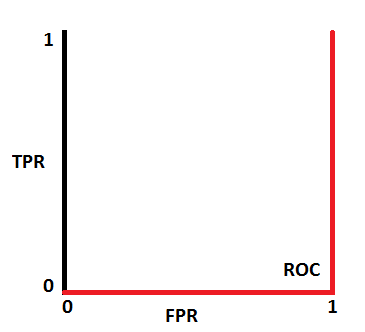
\includegraphics[width=0.3\linewidth]{worst.png}

\end{figure}

\end{itemize}

\textbf{Come costruisco la curva roc?}

Usiamo il classificatore per produrre la classe per ognuna delle istanze che dobbiamo considerare.
Per ognuna delle istanze dobbiamo calcolare la probabilità P(+|A) ovvero la probabilità che il valore predetto sia +. Ora mettiamo in ordine queste probabilità in ordine crescente e per ognuna delle istanze calcoliamo il numero di TP, FP, TN e FN che si ottengono.
Date queste informazioni possiamo calcolare il TPR e il FPR. Per ogni istanza abbiamo un valore di TPR e una di FPR e questo può essere rappresentato come un punto all'interno del piano.

\textbf{Come interpreto la curva roc?}

La curva roc mi mostra il trade-off tra il TPR e il FPR. I classificatori che producono una curva che è più vicina al punto in alto a sinistra sono quelli che hanno una migliore performance.
Più la curva si avvicina alla diagonale dello spazio e meno il modello è accurato sui dati di test.

\begin{figure}[H]
\centering
  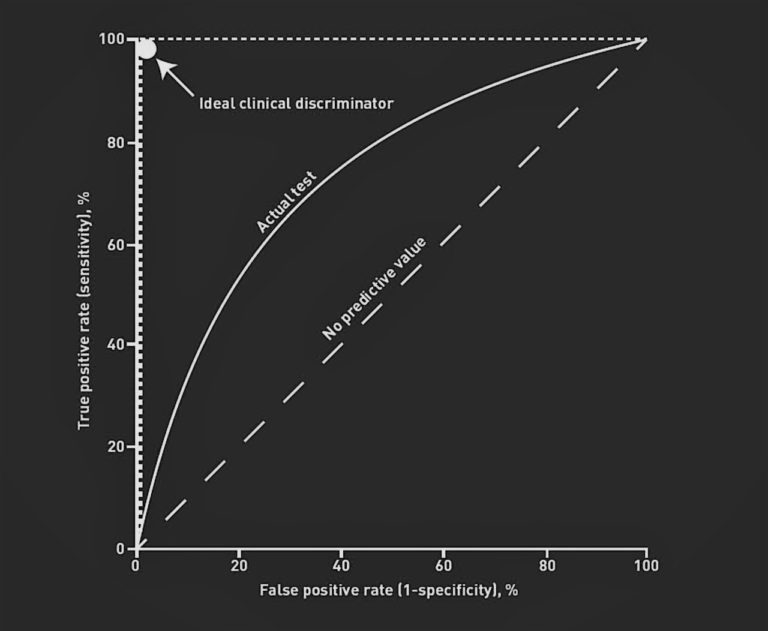
\includegraphics[width=0.7\linewidth]{ROC-curve-1-768x631.jpg}

\end{figure}

Se devo confrontare due classificatori può essere un buon metodo quello di calcolare l'area sotto la curva ROC. 
Un classificatore che ha un'area sotto la curva che è maggiore rispetto all'altro ha più probabilità di classificare male.

\newpage
\chapter{Pattern Mining}

Con Pattern Mining o Association Analysis si intende il procedimento di estrazione di relazioni interessanti tra i dati di un dataset.
Le relazioni che si vogliono estrarre sono quelle più frequenti e quindi non si devono considerare quelle casuali e quelle poco frequenti.
Queste relazioni tra i dati vengono rappresentate tramite dei set, l'obiettivo è selezionare gli item set più frequenti e associare tra loro i set che presentano delle relazioni.

Questi algoritmi di pattern mining possono essere applicati in vari casi, dallo studio delle transazioni in un supermercato per capire quanti prodotti vengono venduti e come fino allo studio dei cambiamenti climatici.

Prendendo il caso delle transazioni della vendita dei prodotti in un supermercato, possiamo rappresentare queste transazioni come una matrice binaria, abbiamo tutti i possibili prodotti e un ID per ogni transazione, per ogni transazione abbiamo un 1 se il prodotto è stato acquistato in quella transazione, altrimenti abbiamo uno 0.

L'insieme di tutti i possibili prodotti è l'insieme I = {$i_1$,..., $i_n$} mentre l'insieme delle transazioni è T = {$t_1$,..., $t_n$}.
Per ogni transazione abbiamo un insieme di prodotti acquistati, quindi, ogni sottoinsieme di I è un itemset e diventa un K-itemset se all'interno dell'itemset sono presenti K prodotti.
Per ogni itemset I, possiamo calcolare:
\begin{itemize}
    \item Support count: contiamo il numero di itemset uguali ad I presenti all'interno del dataset;
    \item Support: $s(I) = \frac{\sigma{(I)}}{N}$ dove I è l'itemset e N è il numero di transazioni, rappresenta il numero di itemset uguali a I nel dataset diviso dal numero complessivo di transazioni. L'itemset viene giudicato frequente se il suo support supera un certo threshold $minSup$.
    Il support deve essere alto e mi dice quanto un itemset è frequente rispetto a tutto il dataset;
    \item Confidence: abbiamo un itemset X e vogliamo capire quanto un itemset Y è legato a X, possiamo scriverlo nella forma $X -> Y$.
    La confidence in particolare mi dice quanto frequentemente i termini in Y compaiono all'interno di X.
    \newline
    $Confidence \ c(X->Y) = \frac{\sigma{(x\ \cup \ Y)}}{\sigma{(X)}}$
    La confidence più è alta e più è probabile che X e Y compaiono insieme.
\end{itemize}

Il supporto lo utilizziamo perchè mi indica quanto effettivamente una association rule è importante rispetto a tutto il dataset, una AR infatti può anche capitare per errore ma dato che noi dividiamo per il numero totale di transazioni, riusciamo a dare uno score più basso a quelle AR che non sono vere. Più il support è alto e più quella regola è importante per il dataset.
Al contrario la confidence misura la probabilità che dato X compaia all'interno dell'itemset anche Y. Più la confidence è alta e più è probabile che Y sia all'interno di una transazione che contiene X.
Trovare tutte le regole che hanno $Support\ > \ minSup$ e $Confidence\ > \ minConf$ non è facile dal punto di vista computazionale ed è espondenziale rispetto al numero delle possibili transazioni.
Quindi per evitare di calcolare support e confidence per ogni transazione, bisogna andare ad utilizzare il pruning per cercare di tagliare alcune transazioni che sappiamo con certezza che non saranno interessanti. Ad esempio se abbiamo un item set che non è molto frequente, tutte le regole che possono essere estratte da quell'item set non saranno a loro volta importanti e non avranno una confidence alta, quindi possiamo tagliarle direttamente.
Quando scegliamo il valore di MinSupp e di MinConf dobbiamo considerare il fatto che:
\begin{itemize}
\item Con un valore troppo alto di MinSupp taglierei fuori troppi itemset che sono frequenti. Con un valore troppo basso invece ne considererei frequenti molti che non lo sono.
\item Con un valore alto di MinConf ho poche regole che vengono considerate valide mentre con un valore basso ne ho molte e alcune di queste non saranno regole davvero valide.
\end{itemize}

L'obiettivo quindi è prima trovare gli itemset più frequenti e poi generare le rule associate all'itemset andando ad estrarre quelle con la maggiore confidence.

Esempio:
\begin{figure}[h!]
  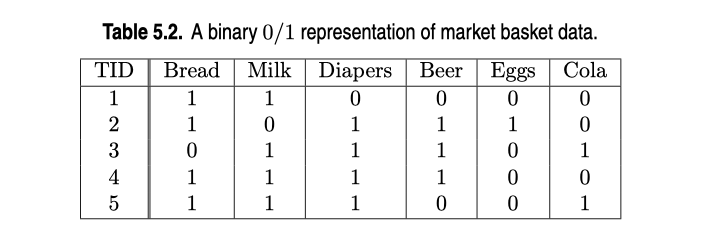
\includegraphics[width=\linewidth]{ConSup.png}
  \caption{Matrice che rappresenta le transazioni}
\end{figure}

Prendiamo l'itemset ${Beer, Diapers, Milk}$ la sua support count è 2, la sua support è $\frac{2}{5}$. La confidence di ${Beer}$ rispetto a ${Diapers, Milk}$ è $\frac{2}{3}$ perchè ho tre transazioni con ${Diapers, Milk}$ mentre ne ho solamente due di queste tre che contengono anche $Beer$.

\section{Generazione degli item set Frequenti}

Se abbiamo un insieme di possibili elementi $I = {i_1,...,i_k}$ allora possiamo generare i corrispondenti $2^k-1$ itemset. Per trovare poi gli itemset più frequenti abbiamo una strategia bruteforce che ci permette di eseguire per ogni transazione il confronto tra l'itemset della transazione e gli itemset generati. Ogni volta che trovo un itemset aumento il suo contatore, alla fine posso avere la lista degli itemset più frequenti. Il problema di questo procedimento brute force è che ha una complessità in termini di tempo che è O(N*M*w) dove N è il numero delle transazioni, M è il numero degli itemset generati e w è la lunghezza del massimo itemset.
Per evitare la procedura bruteforce ci sono vari sistemi che possono essere utilizzati.

\subsection{Metodo Apriori per ridurre il numero di itemset generati}

Per ridurre il numero di itemset che vengono generati possiamo usare il metodo Apriori, in particolare il principio Apriori mi dice che:
\newline    
Se un itemset è frequente allora anche i suoi subset sono frequenti.

Questo principio allo stesso tempo mi dice che se un itemset non è frequente, allora non saranno frequenti neanche tutti gli itemset da cui posso generare quel subset. Esempio, se ${a,b}$ non è frequente, allora non sarà frequente neanche ${a,b,c}$ e quindi quella parte dell'albero la posso andare a non considerare completamente. Questa strategia utilizza il support di un itemset come base per il pruning sfruttando la proprietà che il Support di un certo itemset non potrà mai essere maggiore del Support di un suo subset, questa proprietà si chiama anti monotonicità del support.

\textbf{Complessità}

L'algoritmo Apriori al caso pessimo mi fa generare tutti i vari itemset, quindi, se abbiamo n item iniziali, dovremo generali $2^n$.

\textbf{Funzionamento}

L'algoritmo Apriori per la generazione di itemset frequenti funziona in questo modo:
\begin{itemize}
    \item Al primo step abbiamo i singoli itemset formati da un unico elemento. Per ognuno di questi itemset contiamo il numero delle occorrenze presenti all'interno del dataset, se il numero delle occorrenze è minore di un certo threshold allora non andiamo a considerare quell'itemset.
    \item Al secondo passaggio andiamo a creare degli itemset di 2 elementi partendo dagli itemset di 1 solo elemento che abbiamo preso in considerazione. Anche in questo caso calcoliamo il numero delle occorrenze e poi scartiamo quelle che sono sotto al minSupp.
    La fase di candidate generation deve essere completa, nel senso che dobbiamo generare tutti gli itemset, e deve evitare le ridondanze.
    \item Andiamo avanti in questo modo unendo in itemset via via sempre più grandi fino a quando non rimangono degli itemset frequenti. Ad ogni iterazione dobbiamo generare gli itemset di k elementi stando attenti al fatto che gli itemset generati devono essere formati solamente da subset che sono a loro volta frequenti.
\end{itemize}

L'algoritmo va avanti livello per livello (dell'albero dei possibili itemset) e poi ad ogni iterazione esegue la generazione dei nuovi itemset e testa immediatamente se possiamo considerarli o no.
Da notare che ogni volta che generiamo un nuovo k-itemset partendo dai (k-1)-itemset della precedente iterazione non testiamo di nuovo il supporto di tutti gli itemset generati ma solamente di quelli che crediamo possano essere frequenti, altri invece li scartiamo guardando solamente il supporto dei (k-1)-itemset e quindi rimuoviamo direttamente quelli poco frequenti.

Ogni volta che generiamo un nuovo insieme di itemset e poi scartiamo quelli poco frequenti, ce ne rimangono altri che invece sono frequenti e dobbiamo calcolare per ogni itemset il corrispondente support counting ovvero dobbiamo capire quante volte quell'itemset compare all'interno del nostro dataset.
Controllare in modo brute force tutte le corrispondenze è costoso, quindi dobbiamo trovare una alternativa.
Una prima idea è quella di enumerare tutti i possibili itemset di ogni transazione andando quindi a creare un albero che li contenga tutti. L'albero è un prefix tree e nelle foglie vengono memorizzati i possibili itemset che possiamo generare. Un'alternativa è utilizzare un hash tree.
Con questa struttura dati possiamo prendere l'itemset che abbiamo generato e poi cerchiamo all'interno dell'albero se lo troviamo uno uguale e in tal caso andiamo a modificare il contatore corrispondente di quell'itemset.

\subsection{Complessità}

La complessità dell'algoritmo Apriori dipende da:

\begin{itemize}
    \item Il valore del threshold: se lo mettiamo troppo basso, troppi itemset vengono considerati frequenti e poi dobbiamo calcolare il supporto corrispondente;
    \item Se aumenta il numero di item che possono essere contenuti all'interno dell'itemset aumenta anche l'albero dei possibili itemset che possiamo generare;
    \item Se aumenta il numero di transazioni, aumenta il numero di support counter da memorizzare e quindi lo spazio necessario;
    \item Il tempo di esecuzione dell'algoritmo cresce anche in base alla crescita del numero delle transazioni;
    \item Se le transazioni sono molto lunghe allora aumenta anche la lunghezza media degli itemset e quindi aumenta anche il tempo necessario per il calcolo;
\end{itemize}

\section{Generazione delle association Rules}

Dato un k-itemset è possibile generare delle association rules, se questo viene fatto con un metodo brute force, generiamo fino $2^k-2$ differenti association rules.
Una association rules viene scritta in questo modo: $X->Y-X$ dove Y è l'itemset e X è un subset dell'itemset. In particolare una association rule mi indica che preso un primo subset del nostro k-itemset, esiste un secondo subset del k-itemset che è legato al primo, nel caso delle transazioni al supermercato potrebbe voler dire che quando si acquistano dei prodotti, poi se ne comprano anche altri.
Una association rule può anche avere una correlazione negativa, questo vuol dire che gli item che trovo nella rule non li troviamo spesso insieme all'interno del dataset, ad esempio possono essere prodotti che non vengono spesso acquistati insieme.

Per ogni association rule che viene generata, poi va anche calcolata la confidence corrispondente, questa si calcola così:
\newline
\centerline{$Confidence \ c(X->Y-X) = \frac{\sigma{(X\ \cup \ Y)}}{\sigma{(X)}}$}

In particolare il calcolo della confidence non richiede una ulteriore computazione perchè il support count di X lo abbiamo già calcolato nell'iterazione K mentre il support count di Y-X l'abbiamo calcolato alla iterazione precedente.

Anche per la confidence c'è una proprietà che ci permette di fare il pruning dell'albero andando a tagliare dei subset che non ci interessa prendere in considerazione, non abbiamo però una anti monotono property come avviene con il support.
Per la confidence vale il seguente teorema:
\newline
Teorema: Dato Y, k-itemset e X, subset di Y allora se abbiamo che la association rule $X->Y-X$ ha una confidence che non supera il valore minimo della confidence (minConf) allora possiamo dire che anche prendendo una $X_1$ sottoinsieme di X, l'association rule $X_1->Y-X_1$ non soddisfa la condizione sulla confidence. Quindi per questo motivo possiamo fare il pruning. Ad esempio, dato ${c,b,d}->{a}$ dove $X={c,b,d}$ e $Y-X = {a}$, che non supera minConf, possiamo anche dire che se prendiamo $X_1 = {c,b}$ con $Y-X = {a,d}$ non avremo comunque una association rule che supera il minConf. Quindi possiamo scartare tutte quelle association rule che hanno come postcondizione la ${a}$.

Quando invece dobbiamo generare delle nuove association rules possiamo farlo creando un albero in cui partiamo con delle rule contenenti un solo item, poi andiamo a fare il merge delle varie rules, andando a fare ogni volta il merge di quelle che hanno un prefisso in comune nella post condizione. Esempio, se abbiamo ${cd}->{ab}$ e ${cb}->{ad}$ creiamo una rule ${c}->{abd}$.

\section{Valutazione delle association Rules}

Bisogna saper valutare i pattern che troviamo nei nostri dati, questi pattern devono essere interessanti e devono dirci qualcosa di nuovo riguardo ai dati.
In particolare abbiamo due metodi per giudicare i pattern che abbiamo trovato:

\begin{itemize}
    \item Ci sono delle misure chiamate "Objective Measure of Interestingness" che mi forniscono uno score per i vari pattern che troviamo, alcune di queste misure possono fornire anche delle informazioni statistiche riguardo ai vari pattern.
    \item Il secondo criterio è più legato al tipo di pattern che riusciamo ad estrarre, alcuni patter estratti infatti possono essere del tutto normali e non fornire informazioni aggiuntive mentre altri possono essere più strani e sono proprio questi quelli che vogliamo trovare.
\end{itemize}

Le Objective Measure of Interestingness sono calcolate basandoci sulla tabella di contingenza ed è necessario che l'utente specifichi un threshold per scartare alcuni di questi score.
Con tabella di contingenza si intende una tabella in cui inseriamo i support counter degli item che abbiamo nell'item set del nostro pattern.
Quindi se abbiamo un ${a}->{b}$ dobbiamo fare una tabella di questo tipo:

\begin{center}
    \begin{tabular}{| l | l | l | l |}
    \hline
     & B & \overline{B} &   \\ \hline
    A & f_{11} & f_{10} & f_{1+} \\ \hline
    \overline{A} & f_{01} & f_{00} & f_{0+}\\ \hline
    & f_{+1} & f_{+0} & N\\ \hline
    \hline
    \end{tabular}
\end{center}

Dove $f_{11}$ è il numero delle transazioni dove abbiamo sia A che B, $f_{10}$ è il numero delle transazioni in cui ci sono A ma non B, $f_{01}$ sono le transazioni in cui c'è B ma non A, $f_{01}$ le transazioni dove non ci sono B e A.
Per ogni riga e colonna poi in fondo abbiamo la somma.
Ora partendo da questa tabella possiamo calcolare per ogni 
association rule che generiamo i seguenti score:

Le rule che hanno una confidence alta in alcuni casi possono essere poco utili perchè nella formula della confidence non consideriamo il support dell'elemento che abbiamo come post condizione della rule.

\begin{itemize}
    \item Interest Factor: indica una misura di correlazione tra A e B, il valore assunto può essere 1 se A e B sono indipendenti, minore di 1 se sono negativamente dipendenti e maggiore di 1 se sono positivamente correlati.
    La formula per calcolare l'interest factor è la seguente:
    \newline
    \centerline{$I(A,B)\ =\ \frac{P(A,B)}{P(A)*P(B)}\ =\ \frac{NF_{11}}{F_{1+} + F_{1+}} $}
    Per calcolare P(A,B), P(A) e P(B) dobbiamo prendere il corrispondente valore all'interno della tabella e poi dividerlo per N.
    Ricordare che due eventi si dicono indipendenti se $P(A,B) = P(A)*P(B)$.
    \item Lift: Anche in questo caso è una misura di correlazione che può avere lo stesso valore di Interest Factor.
    La formula per calcolare il Lift è la seguente:
    \newline
    \centerline{$Lift(A,B)\ =\ \frac{P(A,B)}{P(A)} $}
    Se gli eventi sono indipendenti allora Lift = -1.
    \item PS: in questo caso vengono considerate le differenze tra P(A,B) e $P(A)*P(B)$.
    La formula corrispondente è:
    \newline
    \centerline{$PS\ =\ P(A,B) - P(A)*P(B)$}
    \item Correlation Analysis con $\phi$ coefficient: un'altra tecnica utilizzata per analizzare le relazioni tra le coppie di variabili.
    Per le variabili continue la correlazione è definita utilizzando il coefficiente di Pearson.
    Per le variabili binarie la formula è la seguente:
    \newline
    \centerline{$\phi\ =\ \frac{P(A,B)\ -\ P(X)*P(Y)}{\sqrt{P(A)*(1-P(A))*P(B)*(1-P(B))}}$}
\end{itemize}

Per le variabili binarie vale che l'interest factor è uguale alla rule.

\newpage
\section{Metodi alternativi per le association rules}

L'algoritmo Apriori è il primo che è stato usato per la generazione di itemset frequenti, è abbastanza buono e con il pruning riusciamo anche a migliorarne le prestazioni, però ha anche dei problemi e non funziona bene se i dati da analizzare diventano troppi.
Quindi una alternativa che viene utilizzata è l'algoritmo FP-Growth, questo algoritmo utilizza un approccio totalmente differente dal primo e sfrutta un FP-Tree per rappresentare il dataset e trovare gli itemset ricorrenti.

\subsection{Costruire un FP-Tree}

Per utilizzare l'algoritmo FP-Growth è necessario costruire l'FP-Tree corrispondente al dataset.
Questo albero va a comprimere i dati del dataset e viene costruito andando a mappare ogni transazione presente nel dataset all'interno di un path del prefix tree.
Alcuni path dell'albero andranno anche a sovrapporsi e in questo caso andiamo a ridurre lo spazio necessario per memorizzare tutti i dati.
Come viene costruito?
\begin{itemize}
    \item Partiamo con un albero vuoto in cui abbiamo solamente un nodo null. Per ogni transazione presente all'interno del dataset andiamo a creare un path all'interno dell'FP-Tree creando un nodo per ogni elemento dell'itemset. Per ognuno dei nodi che aggiungiamo calcoliamo anche la frequenza, i primi che inserisco hanno frequenza 1.
    \item Andando avanti con le transazioni da inserire nell'FP-Tree troviamo dei path dell'albero che si overlappano con quelle già presenti, in questo caso andiamo ad aumentare la frequenza dei nodi che hanno overlap.
\end{itemize}

Alla fine, dopo aver scansionato tutto il dataset avremo creato un prefix tree che, nel caso ottimo avrà solamente un path perchè tutti gli itemset sono uguali, al caso pessimo avrà tanti path quante sono le transazioni e in questo caso lo spazio occupato sarà anche maggiore della classica tabella con tutte le transazioni. Normalmente diminuiamo lo spazio necessario per rappresentare tutte le transazioni.

Oltre al prefix tree viene anche memorizzata una header table in cui salviamo i puntatori ai vari nodi che troviamo all'interno dell'FP-Tree (il puntatore al primo nodo, poi gli altri nodi con lo stesso label si puntano tra loro da soli).

Per ogni elemento presente all'interno dei vari itemset andiamo poi a calcolare il support corrispondente e ordiniamo gli elementi in base al support crescente per il calcolo dei pattern frequenti mentre la tabella con tutte le transazioni viene ordinata (per ogni transazione) in modo decrescente.
Ordinare prima la tabella non modifica di troppo lo spazio necessario per rappresentare tutto il prefix tree.

\subsection{Algoritmo FP-Growth}

L'algoritmo FP-Growth è un algoritmo che sfrutta la rappesentazione dei dati del dataset in un FP-Tree per estrarre gli itemset più frequenti.
La ricerca di questi itemset più frequenti inizia partendo con gli elementi singoli degli itemset che sono meno frequenti (ad esempio partiamo con e se il support di e è minore di a,b,c,d).
L'algoritmo funziona in questo modo:

\begin{itemize}
    \item Partendo con l'FP-Tree completo andiamo a selezionare tutti i percorsi che comprendono l'elemento che stiamo considerando, diciamo e. Calcoliamo il support count di e e vediamo se è maggiore di minSup. Se è maggiore continuiamo, altrimenti possiamo dire che e non è frequente.
    \item Eliminiamo tutti i path che non comprendono e.
    \item Dato che l'itemset ${e}$ è frequente, dobbiamo vedere se anche ${de,ce,be,ae}$ lo sono. Per farlo dobbiamo costruire un FP-Tree condizionale.
    L'FP-Tree condizionale è simile al normale FP-Tree ma viene utilizzato per trovare gli itemset che terminano con un suffisso particolare.
    Come lo otteniamo:
        \begin{itemize}
            \item Aggiorniamo il support count dei vari nodi dell'albero non prendendo in considerazione i percorsi che non comprendono e.
            \item Quando aggiorno i support vector, alcuni elementi potrebbero non essere più frequenti perchè il loro support count non supera minSup, se ci sono eliminiamo i nodi corrispondenti dal conditional FP-Tree.
            \item Eliminiamo i nodi foglia con l'elemento considerato e quelli che hanno un support count che non supera minSup.
            È importante che prima si ricalcola e poi si elimina.
        \end{itemize}
    \item Una volta costruito il conditional FP-Tree possiamo andare a considerare i percorsi che finiscono con ${de}$. Quindi cancelliamo i nodi che non terminano con de e ricalcoliamo il support count per ${de}$, se è maggiore di minSup allora ${de}$ è frequente.
    \item Ricalcoliamo i support count per gli altri nodi e vediamo se superano il minSup, se non lo superano li togliamo. Quando nell'FP-Tree condizionale rimane solamente un elemento con support $>$ minSup allora possiamo dire che l'itemset che contiene anche quell'elemento è frequente.
\end{itemize}

L'algoritmo va avanti ricorsivamente e funziona nello stesso modo anche per gli altri elementi che dobbiamo prendere in considerazione.

\textbf{Nota su FP-Tree e FP-Grow}:

Rispetto all'algoritmo Apriori per la generazione delle association Rule, l'FP-Tree ha una complessità differente che dipende da quanti percorsi abbiamo nel Tree quindi da quanto possono essere compressi i dati che abbiamo nel dataset.
Se i dati si sovrappongono molto allora possiamo avere un tree piccolo con tanti percorsi sovrapposti, se i dati non sono molto compressi avremo un albero più grande.

Un'altra differenza importante con Apriori è che in Apriori generiamo tutti i possibili itemset e poi cerchiamo di capire se sono frequenti o no, qua invece non devo generarli tutti, ho l'albero e di volta in volta controllo i nodi e vedo se sono frequenti.


\textbf{Esempio}:
\begin{figure}[h!]
  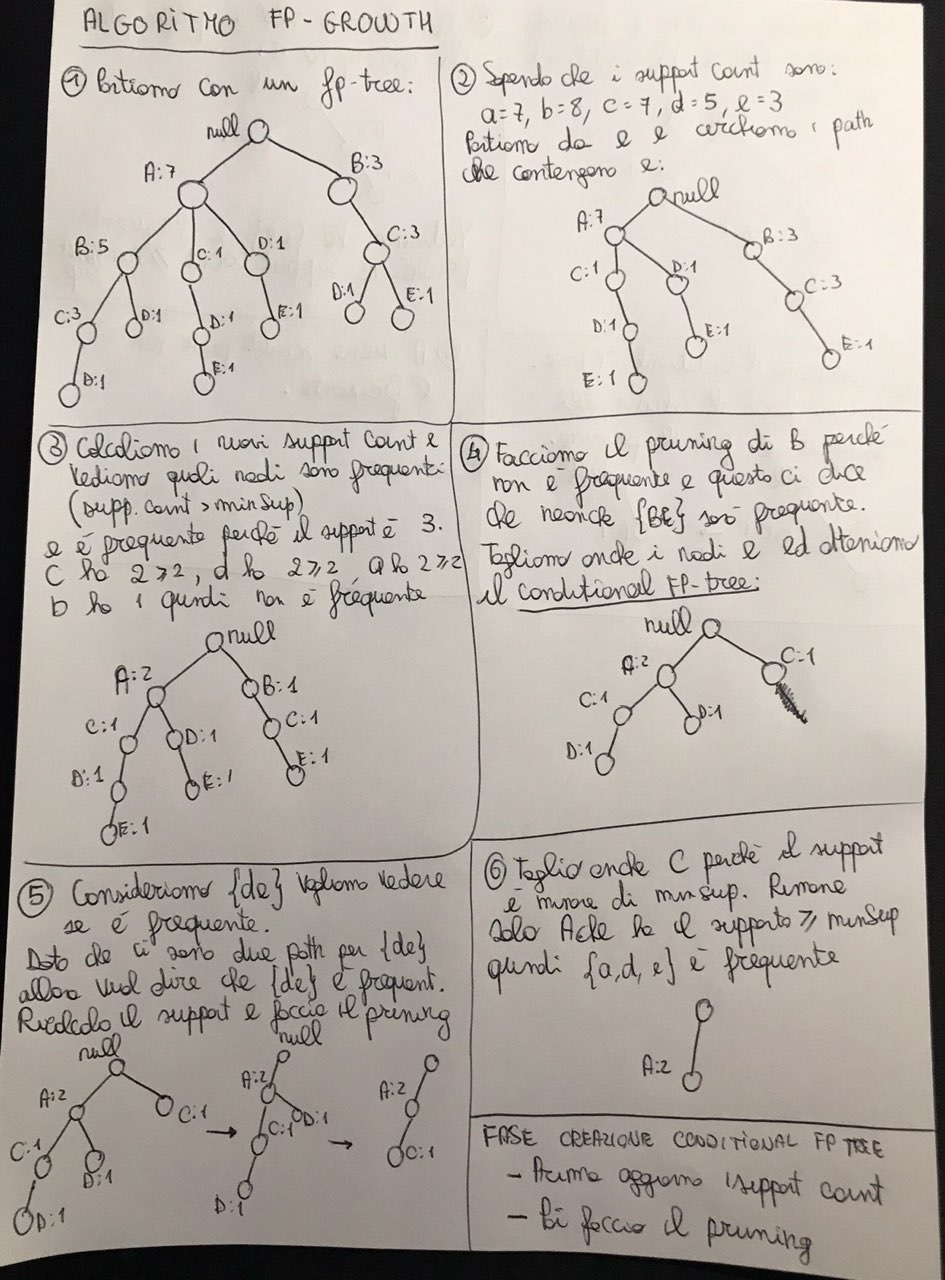
\includegraphics[width=\linewidth]{FPGrowth1.png}
  \caption{Esempio di esecuzione dell'algoritmo FP-Growth con nodo E}
\end{figure}

\begin{figure}[h!]
  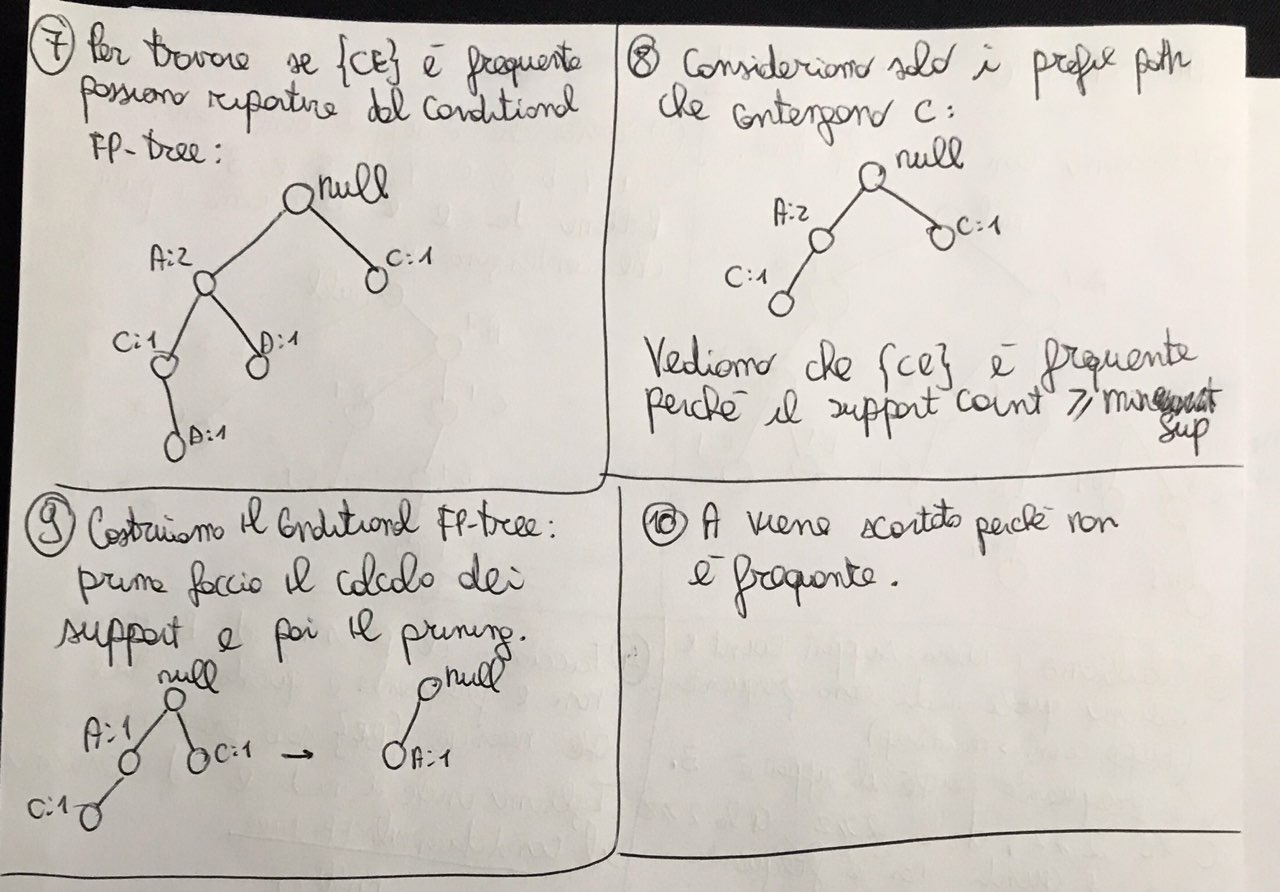
\includegraphics[width=\linewidth]{FPGrowth2.png}
  \caption{Esempio di esecuzione dell'algoritmo FP-Growth con nodo E}
\end{figure}


\chapter{Metodi alternativi per il clustering}

\section{Convergenza e complessità di KMeans}

KMeans è l'algoritmo che usiamo per il clustering, ad ogni iterazione di Kmeans vengono scelti dei centroidi e i punti vengono assegnati ai vari centroidi.
KMeans termina sempre per varie possibilità:
\begin{itemize}
    \item Settiamo un numero massimo di iterazioni
    \item Non cambiano i cluster
    \item Non cambia la posizione dei centroidi
\end{itemize}

Kmeans è un algoritmo che quindi converge sempre e la dimostrazione la possiamo avere se consideriamo il modo in cui giudichiamo l'esecuzione dell'algoritmo. Si usa infatti l'SSE per calcolare la somma delle distanze al quadrato da ogni centroide del cluster.
Per ogni cluster abbiamo un SSE che ci indica la somma delle distanze al quadrato di quel cluster e poi per avere un giudizio complessivo possiamo sommare tutti gli SSE dei vari cluster, questa sommatoria la possiamo chiamare G.
Assegnare ad ogni iterazione i punti ad un nuovo centroide e modificare i cluster contribuisce ad abbassare ad ogni passaggio il valore di G ovvero della sommatoria dell'SSE.
Questo fatto ci indica che prima o poi KMeans converge, anche perchè non possiamo andare sotto allo 0 come valore di G.

La complessità di Kmeans è la seguente:
\begin{itemize}
    \item Per quel che riguarda l'assegnamento dei punti ad un cluster abbiamo $O(k*|P|*|A|)$ dove k indica il numero di cluster, P indica il set dei punti e A è l'insieme degli attributi di ogni punto.
    \item Per l'aggiornamento dei centroidi abbiamo $O(|P|*|A|)$.
    \item Complessivamente abbiamo che la complessità di KMeans è $O(t*k*|P|*|A|)$ dove t è il numero di iterazioni che vengono effettuate
\end{itemize}

\section{Cluster con Mixture Models}

In alcuni casi può essere utile assumere che i dati del dataset sono stati generati come risultati di un processo statistico. Questi dati possono quindi essere descritti utilizzando un modello statistico che li possa fittare. 
Questo modello statistico dovrà essere una distribuzione con i suoi parametri, in base ai parametri il modello fitterà di più o di meno i dati del dataset.
Ad esempio il nostro modello può avere come distribuzione la gaussiana 
\newline
\centerline{$prob(x) = \frac{1}{\sqrt{2\pi}\sigma}e^{-\frac{(x-\mu)^2}{2\sigma^2}}$}

Poi però il modello lo identifichiamo grazie ai parametri che lo contraddistinguono ovvero grazie al vettore $\Theta =(\mu,\sigma)$
L'obiettivo è trovare il miglior modello che fitti i dati ovvero i migliori parametri $\Theta$.

\subsection{MLE: Maximum Likelihood Estimation}

Dato il modello statistico, ad esempio la gaussiana, è necessario poter stimare i parametri di questo modello in modo che fitti al meglio i dati.
Dato un vettore $X = (x_1,...,x_n)$ di valori, vogliamo fittare una gaussiana $N(\mu,\sigma)$ trovando i parametri, la probabilità di osservare un singolo punto è:
\newline
\centerline{$prob(x_i|\Theta) = \frac{1}{\sqrt{2\pi}\sigma}e^{-\frac{(x-\mu)^2}{2\sigma^2}}$}

Mentre la probabilità di osservare tutti i punti, ammesso che siano generati in modo indipendente è:
\newline 
\centerline{$prob(X|\Theta) = \Pi^m \limit_{i=1} \frac{1}{\sqrt{2\pi}\sigma}e^{-\frac{(x-\mu)^2}{2\sigma^2}}$}

L'idea è quella di cercare i parametri $\Theta$ ovvero $\sigma$ e $\mu$ che massimizzano l'ultima formula scritta sopra, questo si chiama Maximum likelihood estimation ovvero MLE.
La probabilità $P(X|\Theta)$ che vogliamo massimizzare è chiamata funzione Likelihood e la possiamo anche esprimere come:
\newline
\centerline{$L(\Theta) = \Pi^m \limit_{i=1} \frac{1}{\sqrt{2\pi}\sigma}e^{-\frac{(x-\mu)^2}{2\sigma^2}}$}

Anche se è più semplice lavorare con il logaritmo della funzione Likelihood:

\centerline{$LL(\Theta) = - \sum^n \limit_{i=1} \frac{(x-\mu)^2}{2\sigma^2} - \frac{1}{2}n\log2\pi - n\log\sigma$}

Quindi in definitiva si cerca di massimizzare la funzione log likelihood $LL(\Theta)$ perchè i parametri che massimizzano questa, massimizzano anche la funzione $L(\Theta)$ perchè il logaritmo è una funzione monotona crescente.
Due parametri che massimizzano $L(\Theta)$:
\newline
\centerline{$\mu = \frac{1}{n}\sum^n \limit_{i=1} x_i $}

\newline
\centerline{$\sigma = \frac{1}{n}\sum^n \limit_{i=1} (x_i-\mu)^2 $}

\subsection{Mixture Models}

Molte volte non mi basta una sola distribuzione per descrivere tutti i dati del dataset, quindi magari ne utilizziamo più di una (anche dello stesso tipo) con vari parametri diversi.
Ad esempio possiamo avere un dataset con le altezze della popolazione, la distribuzione di questi dati è una gaussiana ma i parametri sono differenti a seconda della popolazione che è stata misurata.
Possiamo assumere che all'interno del dataset abbiamo m oggetti $X={x_1,..., x_m}$ e K distribuzioni $j_1,...,j_k$ ognuna con i suoi parametri $\Theta_1,..., \Theta_k$.
Per ogni oggetto $x_i$ possiamo calcolare la probabilità che venga generato eseguendo questi passaggi:

\begin{itemize}
    \item Per prima cosa calcoliamo la probabilità che per generare $x_i$ si sia utilizzata una certa distribuzione. Quindi, ad esempio nel caso dell altezze per nazioni calcoliamo $\pi_G$ e $\pi_C$ che indica la probabilità che $x_i$ sia stato generato con la distribuzione della Grecia o della Cina.
    \item Poi una volta ottenuto il vettore $\Theta=(\pi_G,pi_C, \mu_g,\sigma_g,\mu_c, \sigma_c)$ possiamo calcolare la probabilità di generare $x_i$ dato $\Theta_G$ e dato $\Theta_C$ ovvero calcoliamo $P(x_i|\Theta_G)$ e $P(x_i|\Theta_C)$
    \item Complessivamente possiamo ora calcolare la probabilità di generare $x_i$ ovvero $P(x_i|\Theta)=\mu_g*P(x_i|\Theta_G) + \mu_c*\Theta_C$.
    \item Se poi i vari oggetti presenti in $X$ sono generati in modo indipendente, è anche possibile calcolare la probabilità di tutto l'insieme di oggetti andando a moltiplicare le probabilità dei singoli oggetti:
    \newline
    \centerline{$prob(X|\Theta) = \Pi^m \limit_{i=1} prob(x_i|\Theta)$}
    Questa ultima probabilità è quella che va massimizzata quando andiamo a cercare i parametri $\Theta$ relativi alla distribuzione.
\end{itemize}


Nel modello mixture ogni distribuzione differente descrive un gruppo differente di dati ovvero un cluster.

\subsection{Algoritmo EM}

L'algoritmo EM si basa sul calcolo dell'MLE, parte con una certa distribuzione e con i parametri, per ognuno dei punti presenti all'interno del dataset calcola la probabilità che questo punto appartenga ad una delle distribuzioni. In questo modo l'algoritmo associa un punto ad una distribuzione e quindi assegna i punti ai cluster.
Alla fine viene poi ricalcolato il valore dei parametri della distribuzione.
Nel dettaglio l'algoritmo funziona così:

\begin{itemize}
    \item Partiamo con un set random di parametri $\Theta$
    \item Fino a quando non abbiamo una convergenza (ovvero fino a quando i parametri $\Theta$ non cambiano da un passaggio al successivo) eseguiamo due step, il primo è l'Expectation Step e il secondo è il Maximization Step:
        \begin{itemize}
            \item Expectation: per ogni punto calcoliamo la probabilità \newline $P(Distribuzione D|x_i,\Theta)$ che il punto $x_i$ appartenga ad una certa distribuzione D e assegnamo quel punto al cluste di quella distribuzione;
            \item Maximization: Stimiamo i nuovi parametri $\Theta$ che possono andare a massimizzare la $L(\Theta)$ calcolata nella fase di Expectation. Ogni volta in questa fase cerchiamo di massimizzare la L($\Theta$) rispetto alla vecchia;
        \end{itemize}
\end{itemize}

La fase di expectation corrisponde alla fase di assegnamento dei punti ai centroidi del KMeans, la differenza è che qua l'assegnamento è soft perchè dipende dalla probabilità.
La fase di Maximization corrisponde alla fine di calcolo dei nuovi centroidi svolta in K-Means.

L'algoritmo EM è lento, ha problemi quando ci sono modelli con troppe componenti e quandi il dataset è piccolo, inoltre non è in grado di stimare bene il numero di cluster.
Rispetto a K-Means però è più generale e con l'uso del Mixture model può trovare dei cluster che hanno dimensioni e forme differenti.

\subsection{Miglioramenti per il K-Means}

\subsubsection{Come trovo il numero migliore di K?}

Esiste una variante del k-means che sfrutta il clustering gerarchico, funziona in questo modo:
\begin{itemize}
    \item Creiamo un singolo cluster che contiene tutti i punti e lo inseriamo in una lista
    \item Andiamo avanti fino a che non troviamo K cluster, prendiamo un cluster dalla lista dei cluster e svolgiamo varie iterazioni dividendolo in due cluster utilizzando k-Means. 
    \item Prendiamo la coppia di cluster che abbiamo generato che massimizza l'SSE e la inseriamo all'interno della lista dei cluster.
\end{itemize}

L'algoritmo termina quando abbiamo trovato K cluster, se però K non lo conosciamo l'algoritmo non si ferma fino a che non crea cluster di un solo elemento che sono del tutto inutili.

Per evitare di over-splittare i cluster e ottenere cluster di un solo elemento si usa il BIC.

\subsubsection{BIC: Bayesian Information Criterion}

Si utilizza BIC come criterio di splitting, ad ogni iterazione dell'algoritmo quando devo dividere in due il cluster vado a controllare se il valore dello score BIC dei figli è migliore dello score del padre, se è migliore allora vuol dire che posso andare avanti, se invece non migliora allora non considero quella divisione del cluster.

Questo criterio BIC viene utilizzato nell'algoritmo X-Means:
\begin{itemize}
    \item Diciamo che il valore di K è compreso in un certo range e non può superare una soglia.
    \item Eseguiamo K-Means con il valore minimo di K impostato e andiamo avanti fino a quando la K non supera il valore massimo. 
    \item Ad ogni iterazione divido i punti in K cluster, per ognuno dei cluster però vado a suddividere in due i punti scegliendo due centroidi. Se la divisione migliora lo score BIC allora la lascio e aumento K, altrimenti non la lascio e non aumento K.
\end{itemize}

Xmeans è utile per capire quanti cluster ci sono.


\chapter{Transactional Clustering}

Quando abbiamo un dataset con dati che sono anche categorici non possiamo applicare i classici algoritmi di clustering, tipo K-Means perchè questi lavorano su dati numerici dato che calcolano la distanza tra i vari punti.
Se ad esempio vogliamo clusterizzare i dati di alcune transazioni, e mettere in cluster le transazioni simili allora dobbiamo andare a creare una matrice binaria in cui memorizziamo chi ha comprato cosa.
Se poi volessimo usare K-Means dovremmo prendere la matrice e calcolare le distanze tra i vari vettori che rappresentano le varie transazioni. Il problema è che in alcuni casi andremmo a preferire l'unione di transazioni che non sono simili tra loro semplicemente perchè la distanza euclidea tra i vettori è più bassa delle altre distanze.
Quindi la distanza euclidea e K-Means non sono metodi utilizzabili in questo caso.

\subsection{K-Modes}

Una prima alternativa a K-Means da utilizzare con dati categorici è K-Modes, in questo caso l'obiettivo dell'algoritmo è minimizzare:
\newline
\centerline{$P(W,Q)=\sum^k \limit_{l=1} \sum^n \limit_{i=1} w_{i,l}d(X_i,Q_l)$}
Abbiamo a disposizione un dataset X di oggetti, poi W è la matrice in cui memorizziamo l'appartenenza di un vettore ad un cluster, Q è l'insieme dei cluster, x è l'insieme dei vettori in cui rappresentiamo il "carrello" e $d(X_i,Q_l)$ è la funzione che utilizziamo per calcolare la distanza.
In particolare per ognuno dei cluster abbiamo un centroide che rappresenta il cluster. Questi centroidi vengono salvati all'interno del vettore Q.
In k-modes la funzione $d(X_i,Q_l)$ che calcola la distanza tra i vari cluster e un vettore che dobbiamo assegnare esegue il calcolo del numero dei mismatch tra i due vettori e alla fine assegna il vettore al cluster con la mode più simile.
L'algoritmo funziona in questo modo:
\begin{itemize}
    \item Selezioniamo gli oggetti che inizialmente fanno da mode (ovvero andiamo a prendere come rappresentanti gli oggetti che hanno gli attributi più frequenti);
    \item Assegnamo gli oggetti ai vari cluster misurando la "distanza" dalla mode, la distanza viene misurata in base al numero dei mismatch tra il rappresentante del cluster e l'oggetto da assegnare;
    \item Ri-calcoliamo la mode dei vari cluster andando a prendere come centroide il valore che è formato dagli attributi più frequenti.
\end{itemize}

Esempio di calcolo del centroide:
Abbiamo un cluster: ${BPH,BRT,BPH}$ il centroide è BPH perchè B compare in tutti e tre, P compare due volte e H compare due volte.
Se invece abbiamo ${APH,APT,ARH,ART}$ il centroide diventa APT, A è comune in tutti, gli altri due attributi invece hanno la stessa frequenza in tutti gli attributi quindi ne prendo uno a caso.

\subsection{Rock ����}

Un secondo algoritmo per la clusterizzazione di dati categorici è Rock, in questo caso si tratta di un algoritmo per il clustering gerarchico. Rock utilizza per il clustering due concetti:
\begin{itemize}
    \item Neighbours: l'idea dei neighbours è quella di andare a vedere le somiglianze tra due oggetti, quindi tra due vettori o tra un vettore e un cluster. La somiglianza in questo caso viene calcolata utilizzando lo score Jaccard $\frac{A\ \land \ B}{A\ \cup \ B}$. Questo concetto ci permette di capire quali sono i vettori più simili senza dover calcolare la distanza tra i vettori. In questo caso viene catturata la somiglianza locale. A e B sono simili se lo score della somiglianza supera una certa threshold.
    \item Links: Partendo dalla matrice in cui andiamo a scrivere lo score della similarità calcolata con la jaccard andiamo a creare una lista di neighbour ovvero elenchiamo i vicini dei vari "nodi". Possiamo poi calcolare il numero di vicini che sono in comune tra due oggetti. Il link cattura la somiglianza globale all'interno del grafo con tutti i nodi.
    Presi due oggetti A e B possiamo calcolare il link con la seguente formula (indica quanti sono sia vicini di A che di B):
    \begin{equation}
        link(A,B) = |neighbor(A) \land neighbor(B)|
    \end{equation}
\end{itemize}

Neighbours e Links mi forniscono una misura globale di somiglianza tra vettori in modo da capire come clusterizzare.
Questa misura di somiglianza è la seguente e va massimizzata:
\newline
\centerline{$E_l = \sum^K \limit_{i=1} * \sum \limit_{p_q,p_r \in C_i}\frac{link(p_q,p_r)}{n_i^{1+2f(\Theta)}}$}

Dato che Rock è un algoritmo di clustering gerarchico, vanno uniti i vari cluster a vari livelli, per capire quali sono i cluster da unire e quando vanno uniti devo calcolare uno score che dipende dal link score dei vari cluster e da altri fattori:

\begin{equation}
    g(C_i,C_j) = \frac{link(C_i,C_j)}{(n_i + nj)^{1+2f(\Theta)}-n_i^{1+2f(\Theta)}-n_j^{1+2f(\Theta)}}
\end{equation}

Dove $f(\Theta) = \frac{1-\Theta}{1+\Theta}$, $n_i$ è la cardinalità del cluster $C_i$.
Quindi per ogni possibile coppia di cluster andiamo a calcolare questo score e vediamo quali sono i cluster che vanno uniti prima.

Algoritmo:

In input abbiamo i dati da clusterizzare, la threshold della similarity e il numero di cluster che vogliamo trovare.

\begin{itemize}
    \item Per prima cosa costruiamo un random sample dei dati partendo dal dataset iniziale, questo perchè altrimenti avremmo troppi dati, quindi prima troviamo i cluster con pochi dati e poi gli altri li inseriamo nei vari cluster creati.
    \item Inizialmente partiamo con un cluster per ogni punto, dobbiamo misurare la distanza tra ogni coppia di cluster e trovare quelli che sono da unire, per capire quali unire usiamo la misura di somiglianza vista in precedenza.
    Questo calcolo della distanza lo svolgo più di una volta fino a quando non mi fermo per una condizione di stop.
    \item I punti che non sono nel random sample e che non sono labellati vanno assegnati ai vari cluster.
\end{itemize}

Come si fanno gli esercizi su ROCK:

\begin{itemize}
    \item Abbiamo inizialmente un elenco di vettori in cui troviamo i vari oggetti e poi abbiamo una threshold $\Theta$
    \item Calcoliamo la jaccard similarity tra i vari vettori e creiamo una matrice in cui inseriamo questi valori della similarity
    \item Partendo dalla matrice della similarity scartiamo quelli che sono sotto la threshold e creiamo per ogni vettore l'elenco dei suoi neighbour.
    \item Poi creiamo una seconda matrice in cui memorizziamo i link tra i vari vettori ovvero andiamo a vedere quali sono i neighbour in comune tra i vari vettori
    \item Calcoliamo il link score tra i vari vettori e li uniamo per formare i cluster creando poi il dendrogramma.
\end{itemize}

\subsubsection{Nota}

L'algoritmo Rock è in grado di vedere somiglianze "globali" tra le varie transazioni, questa è una differenza rispetto al clustering gerarchico.
Nel clustering gerarchico infatti calcoliamo la distanza tra i due punti e poi uniamo quelli più vicini, qua calcoliamo la distanza tra i vettori ma poi uniamo quelli che hanno più vicini in comune, quindi è una somiglianza più globale.

\subsection{CLOPE}

Altro metodo per clusterizzare dati con attributi categorici, funziona specialmente con dataset molto grandi.
L'idea di questo algoritmo è quella di andare a massimizzare l'overlapping tra i set di dati che si trovano all'interno dello stesso cluster. 
Avremo quindi una funzione che mi calcola questo overlap e dovremo preferire i cluster che hanno un valore più alto di overlap.

Supponiamo di avere un database con delle transazioni, vogliamo fare un confronto tra due possibili clusterizzazioni che abbiamo creato. Partendo dai cluster possiamo andare a creare un istogramma (contando il numero di occorrenze dei vari termini) in cui possiamo calcolare l'altezza e la larghezza.
La size S del cluster indica il numero totale di attributi del cluster C, la larghezza W del cluster indica il numero di attributi differenti che troviamo all'interno del cluster, l'altezza invece è la media tra la size e la larghezza ed è definita come: 
\begin{equation}
    H(c) = \frac{S(c)}{W(c)}
\end{equation}

Presi i due cluster quindi possiamo andare a calcolare il profit:

\begin{equation}
    Profit_r(C) = \frac{\sum^k \limit_{i=1} \frac{S(C_i)}{W(C_i)^r}* |C_i|}{\sum^k \limit_{i=1} |C_i|}
\end{equation}

Dove la r è chiamata repulsion e (dovrebbe essere tipo un valore che negli esercizi viene dato oppure è il numero di cluster da confrontare) se è grande allora le transazioni nello stesso cluster devono condividere una grande porzione di elementi.

\subsection{COOLCAT}

Algoritmo per il clustering di dati categorici che sfrutta l'entropia per clusterizzare. Per ogni cluster viene calcolata l'entropia e si va a preferire quei cluster che hanno una entropia più bassa perchè vuol dire che sono più puri e quindi che i dati presenti all'interno sono simili tra loro. In questo caso non calcoliamo la distanza tra i vettori.
Quindi, dato un dataset con n oggetti l'obiettivo è quello di creare K cluster partizionando gli oggetti e minimizzando l'entropia di ognuno di questi cluster.
Come funziona l'algoritmo:

\begin{itemize}
    \item Inizialmente partiamo con una parte dei dati del dataset, scegliamo una quantità S di dati minore di D che è il totale.
    \item Troviamo un set iniziale di vettori facendo in modo che l'entropia tra di essi sia massimizzata, questi sono i cluster iniziali
    \item Ora assegno ogni punto ad un cluster e creo i cluster
    \item Ogni punto di D viene assegnato ad un cluster facendo in modo che, a seguito dell'assegnamento l'entropia del cluster vada a diminuire.
\end{itemize}

\subsection{TX-Means}

Tx-Means è un algoritmo che ci permette di clusterizzare in modo efficiente i dati categorici in particolare quando dobbiamo applicarlo più volte a differenti dataset. Ad esempio lo applichiamo più volte a vari dataset quando dobbiamo andare a suddividere il dataset in base al cliente e per ogni cliente abbiamo tante transazioni.
Non ha come parametro il numero di cluster da creare, quindi ad ogni iterazione va a dividere in cluster andando a controllare tramite il bic score quando fermarsi.
L'algoritmo TX-Means termina per ogni input, la complessità è O(It*N*K*D) dove It è il numero di iterazioni, N è il numero di transazioni in input, D è il numero di elementi nel dataset e K è il numero di cluster che vengono generati.

\chapter{Privacy}

Quando si analizzano dati c'è da considerare il fatto che anche un data scientist dovrebbe tenere in considerazione aspetti legati all'etica e alla privacy.
Quando si analizzano i dati abbiamo due concetti importanti legati all'anonimicità:
\begin{itemize}
\item Anonymized data: avere dei dati anonimizzati mi garantisce che non sarà possibile risalire alla persona a cui appartiene quello specifico dato.
\item PseudoAnonymized data: avere dei dati pseudo anonimizzati mi dice che per risalire alla persona a cui appartengono quei dati ho necessità di altre informazioni aggiuntive.
Per esempio per garantire la pseudo anonimicity devo sostituire quei valori che sono identificativi della persona con un valore che sarà comunque univoco ma che non mi fa identificare direttamente la persona. Ad esempio potrei sostituire la coppia nome, cognome con un ID. Questo valore che scelgo per sostituire il nome non deve essere essere reversibile senza avere altre informazioni che mi associano quel valore con il nome corretto.
\end{itemize}

Nonostante questa suddivisione non è possibile dire che i dati pseudoanonimizzati sono sufficienti per garantire una protezione dei dati. Infatti anche se i dati sono pseudoanonimizzati, rimangono comunque dati personali.
Ad esempio se abbiamo una lista di persone che possono votare alle elezioni e una lista di pazienti di un ospedale possiamo fare una join tra dati che non sono identificativi per ottenere comunque una lista più piccola di persone che possono essere legate alla lista di pazienti.

All'interno di un database i vari attributi possiamo suddividerli tra:
\begin{itemize}
\item Identificativi
\item Quasi identificativi
\item Sensibili 
\end{itemize}

Un concetto importante è quello di K-Anonymity ovvero quando abbiamo a disposizione un database e dei dati vorremmo che ogni riga della tabella fosse "nascosta" tra le altre k-1 nel senso che date alcune informazioni non voglio poter trovare direttamente la riga della tabella che più si avvicina a quello che cerco. Ad esempio se nella tabella ho data di nascita e zip code e faccio una ricerca di data di nascita e zip code trovando 2 righe della tabella non va bene perchè ho perso di nuovo la pseudoanonymicity.
Quindi una possibile soluzione potrebbe essere quella di generalizzare ancora di più i dati che trovo nella tabella oppure sopprimere alcuni che non servono o che sono outlier.
Un'altra possibile soluzione è la randomizzazione dei dati che troviamo nella tabella.

Quando poi si fa una query in un database con dati sensibili si dovrebbe aggiungere del rumore alle risposte che vengono fornite in modo tale da avere delle risposte che non mi possono far ottenere informazioni che riguardano gli altri dati della tabella.

\textbf{Il data mining può violare la privacy?}

Ci sono tecniche come ad esempio la ricerca delle association rules che può essere un problema per la privacy.

Quando si parla di privacy by design si intende l'idea di garantire la privacy fin dal momento iniziale in cui il dato viene creato.
Quindi serve un framework che sia in grado di rendere anonimi i dati garantendo comunque la possibilità di eseguire delle query.
Con Privacy risk measure invece si intende la probabilità di re-identificare una persona dati i dati che troviamo nel database.
Questo rischio di essere identificato viene rappresentato in un grafico che è la curva Rac.

\textbf{Predire i rischi per la privacy degli individui}

Possiamo sviluppare un classificatore che predice se un individuo è a rischio per la privacy o no. Se abbiamo i dati possiamo allenare un classificatore in modo tale che i dati che inserirò successivamente potranno essere studiati in automatico per predire il rischio.



\chapter{Advanced Classification Methods}

\section{Instance Based-Classifiers}

In questo caso l'idea è quella di effettuare una classificazione andando a memorizzare gli esempi di training utilizzandoli poi per fare previsioni su record non labellati.
Abbiamo due metodi.

\subsubsection{Rote-learner}

Metodo molto limitato perchè memorizza tutto il training set poi quando vede un nuovo record da classificare va a controllare se uno degli esempi del training set è del tutto identico e in tal caso prende la stessa classe.

\subsubsection{Nearest Neighbor}

Generalizzazione del Rote Learner, in questo caso però non vado alla ricerca dell'esempio identico a quello da classificare.
L'idea è di andare a prendere k esempi che sono i meno distanti da me e poi scegliamo la classe che maggiormente classifica questi k esempi.
L'algoritmo per funzionare necessita in input del set degli esempi di training, di una matrice delle distanze in cui memorizzare le distanze tra i punti e il valore di k che mi dice quanti punti devo considerare per classificare il punto.

Per classificare:
\begin{itemize}
    \item Prima di tutto prendo K punti che sono i più vicini a me, la vicinanza tra i punti la calcolo ad esempio con la distanza euclidea;
    \item Assegno al record che vogliamo classificare la classe che compare maggiormente nei K vicini basandomi anche sulla distanza dei vicini da me.
\end{itemize}

La scelta della K è importante, se scelgo un valore troppo piccolo vuol dire che sarò troppo soggetto al rumore, con una k troppo grande invece andrei a considerare anche dei punti che appartengono ad altre classi e non sono troppo simili a me.
Per il calcolo della distanza tra i vari punti c'è anche un'altra cosa da considerare, non vogliamo che un certo attributo vada ad essere predominante nel calcolo della distanza, quindi è necessario che il vettore venga normalizzato.

K-NN è un algoritmo per la classificazione che non crea un modello vero e proprio come può essere un albero, per fare le previsioni abbiamo sempre la necessità di avere il dataset, quindi questo è un primo problema. Abbiamo poi un secondo problema perchè la fase di previsione necessita del tempo.

\section{Classificazione Bayesiana}

Si tratta di un classificatore che utilizza la probabilità per assegnare una certa classe ad un record che non abbiamo ancora visto nel dataset di training.
In particolare per la classificazione si basa sul teorema di Bayes, per enunciarlo consideriamo prima la probabilità condizionale:
\begin{equation}
    P(C|A) = \frac{P(A,C)}{P(A)}    
\end{equation}

\begin{equation}
    P(A|C) = \frac{P(A,C)}{P(C)}
\end{equation}

Quindi il teorema di Bayes mi dice che:
\begin{equation}
    P(C|A) = \frac{P(A|C)P(C)}{P(A)}
\end{equation}

Questa uguaglianza vale perchè il termine $P(A,C)$ è uguale a $P(A|C)P(C)$ e questo lo ricavo della seconda probabilità condizionale.

Quindi per usare il classificatore Bayesiano devo calcolare per prima cosa la probabilità delle varie possibili classi che abbiamo nel dataset. Poi per ogni attributo prendiamo il possibile valore e calcoliamo la probabilità condizionale che valga quel valore sapendo che la classe del record è una o un'altra.
Esempio:
\begin{itemize}
    \item Calcolo per prima cosa la probabilità $P(Yes)$ e $P(No)$ che sono le probabilità delle possibili classi
    \item Per ogni attributo calcolo la probabilità condizionale, ad esempio per l'attributo temperatura calcolo le probabilità $P(Alta|Yes)$, $P(Media|Yes)$, $P(Bassa|Yes)$ e faccio la stessa cosa anche per il no.
\end{itemize}

Quando devo classificare una nuova istanza:

\begin{itemize}
    \item Abbiamo un record con gli attributi $A_1...A_n$. devo calcolare la probabilità a posteriori che vale:
    \begin{equation}
        P(C|A_1,...,A_n) = \frac{P(A_1,...,A_n|C)P(C)}{P(A_1,...,A_n)}
    \end{equation}
    \item Cerco il valore di C che massimizza $P(C|A_1,...,A_n)$
    \item Il valore C che massimizza è identico anche se calcoliamo $P(A_1,...,A_n|C)P(C)$. 
\end{itemize}

Se ho due classi, si e no calcolo questa probabilità due volte e poi assegniamo al record la classe per cui abbiamo ottenuto la probabilità maggiore.
Esempio:
\begin{equation}
    P(X|Yes)P(Yes) = P(rain \land not \land high \land false|Yes)*P(Yes)
\end{equation}

\subsection{Naive Bayes Classifier}

Oltre al metodo di Bayes possiamo classificare utilizzando le probabilità anche utilizzando il metodo Naive Bayes.
La differenza tra i due è che questo secondo metodo è Naive perchè qua noi assumiamo che gli attributi siano indipendenti tra loro.
L'indipendenza degli attributi ci permette di calcolare la probabilità come un prodotto e non calcolando tutto insieme:
\begin{equation}
P(A_1,...,A_n | C) = P(A_1 | C) * ... * P(A_n | C)
\end{equation}

Con questo classificatore abbiamo un problema perchè c'è la possibilità che una di quelle probabilità vada a 0, in questo caso ci troviamo con tutta la probabilità condizionale che va a 0.
Per risolvere il problema possiamo calcolare la singola probabilità che normalmente calcoleremmo come $P(A_i|C) = \frac{N_{ic}}{N}$ utilizzando la formula di Laplace che non mi manda a 0 la probabilità perchè usiamo un +1 al numeratore e un +c (dove c è il numero delle classi) al denominatore. Quindi con Laplace la probabilità diventa:
\begin{equation}
P(A_i | C) = \frac{N_{ic}+1}{N_c + c}
\end{equation}

Naive Bayes quindi è in grado di gestire missing values e attributi irrilevanti, però potrebbe non essere troppo ben funzionante se assumiamo l'indipendenza tra attributi che in realtà non sono indipendenti.

\section{Ensemble Methods}

L'idea dell'Ensemble Methods è di suddividere il dataset in tanti dataset più piccoli, per ogni dataset creiamo un classificatore differente e poi alla fine uniamo tutti questi classificatori "base" in un unico classificatore che utilizziamo per classificare le istanze di test. 
Questa unione di classificatori ha un error rate minore dei singoli classificatori "base".
Ci sono due metodi per generare dei classificatori ensemble, il bagging e il boosting.

\subsection{Bagging}

Partendo dai dati iniziali vengono fatti dei sample dei dati, dato che la dimensione del dataset rimane costante, alcuni dei dati verranno ripetuti più di una volta perchè si fa un replacement dei dati.
Per ognuno di questi sample che creiamo possiamo poi creare un differente classificatore.
Ogni sample ha probabilità $(1-\frac{1}{n})^n$ di essere selezionato.

\subsection{Boosting}

Si tratta di una evoluzione del bagging in cui però non andiamo a prendere ogni volta i dati random ma assegniamo dei pesi. 
Inizialmente i pesi saranno tutti uguali per ogni elemento del dataset, poi successivamente a mano a mano che creo nuovi dataset svolgo la classificazione, assegno dei pesi più alti quando un certo record non viene classificato bene.
Quindi negli step successivi succederà che quel record che non ho classificato bene e che quindi ha un peso più alto verrà scelto di nuovo per essere inserito all'interno dei successivi dataset sample.

\subsection{Rule-Based Classifier}

Si tratta di classificatori che utilizzano una serie di regole if... then.
Partendo da una serie di condizioni andiamo a classificare il nostro record e gli assegniamo una classe.
Le regole che vengono create devono essere mutuamente esclusive in modo che ogni record venga coperto solamente da una regola e devono essere esaustive nel senso che tutte le possibili combinazioni devono essere considerate, ogni record del training set deve essere coperto da almeno una regola.

Se abbiamo un record non classificato, controlliamo se gli attributi contenuti al suo interno matchano una qualche regola di quelle che abbiamo creato e in tal caso assegniamo una classe.
Per il rule-based classifier possiamo definire due metriche di giudizio:
\begin{itemize}
    \item Coverage: mi indica la percentuale di record che soddisfano la precondizione di una regola. Ad esempio se abbiamo 10 record e abbiamo che 4 di questi soddisfano la precondizione $Sposato\ =\ Si$ allora la coverage sarà del $40\%$;
    \item Accuracy: mi indica la percentuale di record che soddisfano la post condizione di una regola. Qua ad esempio se abbiamo 4 record che soddisfano la precondizione e 2 che soddisfano la post condizione possiamo dire che l'accuracy è del $50\%$ perchè abbiamo $\frac{2}{4}$.
\end{itemize}

Le regole possono essere generate partendo da un albero di decisione e seguendo tutti i possibili percorsi. Per ogni possibile percorso avremo una regola. Alcune di queste regole possono essere anche semplificate, la semplificazione di una regola comporta però l'assenza della mutua esclusione tra le varie regole e inoltre le regole non sono più mutuamente esclusive. La perdita della mutua esclusione la possiamo risolvere ordinando le regole in base al rank delle singole query oppure in base alla classe (ad esempio prima tutti i No poi tutti i Si) mentre la perdita di esaustività la possiamo risolvere inserendo una regola di default che viene utilizzata se nessuna delle precedenti regole matcha il record che vogliamo classificare.

Avendo a disposizione dei dati come facciamo a creare le rules?

\subsubsection{Metodo Diretto per creare le rules}

Il metodo diretto prevede questi passaggi per creare le varie rules:
\begin{itemize}
    \item Iniziamo da una regola vuota ${}$.
    \item Fase di rule growing. Aumentiamo il contenuto della rule usando la funzione Learn One Rule.
    \item Eliminiamo gli esempi di training coperti dalla rule. Questo passaggio è necessario perchè altrimenti avremmo delle rule identiche a quella che abbiamo appena inserito, invece in questo modo non abbiamo ripetizioni.
    \item Torniamo allo step 2 e ripetiamo fino a quando non matchiamo uno dei criteri di stop, ad esempio controlliamo se il gain che abbiamo ottenuto con la nuova regola è significativo o no.
\end{itemize}

Per la fase di Rule Growing abbiamo due possibilità, l'algoritmo CN2 (ogni volta sceglie l'attributo che minimizza l'entropia nella rule) che parte da un congiunto vuoto ${}$ e l'algoritmo Ripper (ogni volta sceglie l'attributo che massimizza l'information gain della rule).
In questo caso per creare le rules abbiamo delle metriche che mi permettono di giudicare la creazione di nuove rules:
\begin{equation}
    Accuracy = \frac{n_c}{n}
\end{equation}

\begin{equation}
    Laplace = \frac{n_c + 1}{n + k}
\end{equation}

\begin{equation}
    M-estimate = \frac{n_c + k*p}{n + k}
\end{equation}

Uno dei metodi diretti è ripper che si comporta in questo modo:
\begin{itemize}
    \item Per un problema che deve classificare solamente due classi, prendiamo una delle due classi, ad esempio Si e creiamo le regole corrispondenti. Per l'altra classe invece, ad esempio "no" creiamo una classe di default che ci porta tutti i record in no.
    \item Per un problema di classificazione con più di una classe invece dobbiamo ordinare prima le classi in base al numero di apparizioni, poi dopo classifichiamo prima quelli che compaiono meno volte e poi sul set che rimane prendiamo di nuovo la classe che compare di meno.
\end{itemize}

\subsubsection{Metodi Indiretti per creare le rules}

In questo caso prendiamo un decision tree a cui non è stato fatto il pruning e poi creiamo le regole corrispondenti.

I vantaggi del rule-based Classifier:
\begin{itemize}
    \item Espressivo come il decision tree
    \item Facile da interpretare
    \item Facile da generare
    \item Può classificare istanze rapidamente
    \item Le performance sono comparabili al decision tree
\end{itemize}

\chapter{Wisdom of Crowd e Ensemble Learning}

Secondo l'idea del Wisdom of Crowd, la conoscenza collettiva di un gruppo di persone diverse e indipendenti supera la conoscenza di un individuo singolo. 
Abbiamo una domanda che viene posta alle persone che formano il "crowd" (la folla) e ognuno all'interno della folla vota in base a quello che pensa, la folla sarà composta dal 30\% di persone esperte sull'argomento e dal 70\% di persone che invece non sono esperte.
Possiamo quindi calcolare subito la probabilità della previsione corretta svolta da una persona esperta o da una persona che non è esperta, conoscendo questi valori poi possiamo calcolare la probabilità che preso un qualsiasi utente all'interno della folla, possa fare una previsione corretta.
\begin{equation}
    P(previsione corretta | esperto) = p_e
\end{equation}

\begin{equation}
    P(previsione corretta | Non esperto) = p_{ne}
\end{equation}

\begin{equation}
    P(previsione corretta | Utente nella rete) = 0.3*p_e + 0.7*p_{ne}
\end{equation}

Come risposta della folla consideriamo la media di tutte le risposte. Vogliamo una folla formata sia da esperti che da non esperti per vari motivi:
\begin{itemize}
    \item Se prendiamo una folla abbastanza grande, ci saranno sicuramente degli esperti all'interno
    \item Non vogliamo che la risposta sia totalmente influenzata dagli esperti
    \item Per alcune domande potrebbe essere difficile trovare più di un set di esperti
\end{itemize}

Ci sono poi varie regole per formare una folla che possa fornire delle risposte adeguate alle domande:
\begin{itemize}
    \item Le persone nella folla devono avere differenze per quanto riguarda l'educazione e le opinioni.
    \item Le persone nella folla devono essere indipendenti e non devono influenzarsi l'una con l'altra, nessuna copia le altre.
    \item Le persone devono conoscere un certo ambito.
    \item Deve esserci un modo per aggregare tutte le previsioni in una sola previsione.
\end{itemize}

\section{Wisdom of Crowd e Machine Learning}

Vogliamo utilizzare il sistema del Wisdom of Crowd nel campo del Machine Learning, in questo modo quello che vorremmo fare è utilizzare vari modelli che mi fanno delle previsioni e poi vogliamo combinare i risultati forniti da questi modelli per ottenere un risultato finale.
Per un classificatore definiamo il bias come la differenza al quadrato tra la media delle funzioni stimate e la funzione reale.
\begin{equation}
    Bias = (E[f\^(x)] - E[f(x)])^2
\end{equation}

Il bias è basso quando il modello è molto complesso e si adatta molto ai dati, quando invece il modello è meno complesso allora il bias è più alto. Noi vogliamo che il bias venga mantenuto basso.
Se però abbiamo tanti classificatori con un bias alto, possiamo unirli insieme con la tecnica Ensemble vista in precedenza per andare ad ottenere un classificatore che ha un bias basso.
Per utilizzare l'Ensemble Prediction è necessario che i classificatori siano sufficientemente indipendenti.

Preso un classificatore poi possiamo definire anche la varianza come la media della differenza al quadrato della previsione che ci attendiamo e la media delle previsioni dei vari classificatori.
\begin{equation}
    Varianza = E[(f\^(x) - E[f\^(x)])^2]
\end{equation}

In questo caso un modello molto complesso ha anche un'alta varianza perchè se il modello è complesso vuol dire che è molto legato ai dati di training e quindi si distacca molto dal valore medio che ci aspettiamo come risultato della classificazione. Un modello poco complesso ha anche una bassa varianza, praticamente il contrario del bias.
Quello che vogliamo quindi è un modello con un bias basso e una varianza bassa.

\subsection{Ensemble Method: Boosting}

Si tratta di un metodo che partendo da dati di training S in cui ogni record ha anche un suo label, va a creare in modo iterativo dei classificatori $h_1$...$h_t$ dove ognuno di questi classificatori viene inserito all'interno di un insieme H.
Per ognuno degli esempi di training mantengo anche un peso che aumenta o diminuisce a seconda della capacità di classificare quel record. Se classifico male il record allora il peso aumenta, se invece lo classifico bene diminuisce.
Ad ogni iterazione dell'algoritmo produco un modello, alla fine quando dovrò fare una previsione considero tutti i vari modelli che sono stati creati e sommo la previsione di ognuno di questi modelli, questa somma finale mi indica la previsione per quel record.
Alla fine della classificazione ottengo il miglior classificatore.
Questo algoritmo per la classificazione ha delle proprietà interessanti:
\begin{itemize}
    \item L'errore sul training può anche tendere a 0
    \item Il classificatore che viene creato in questo modo ha una buona generalizzazione, ci aspetteremmo un over-fitting ma in realtà non c'è.
    \item Il motivo per cui non va in overfitting è legato al fatto che anche quando arriva ad un modello che è in grado di classificare correttamente tutti i dati di training si cerca comunque di massimizzare il margine del classificatore, in modo che quando andiamo a provare i dati di test abbiamo comunque una buona classificazione. 
\end{itemize}

\subsection{Ensemble Method: Bagging}

I decision tree sono dei classificatori che hanno un bias molto basso perchè producono dei decision boundery molto precisi, allo stesso tempo però hanno anche un'alta varianza perchè sono molto dipendenti dai dati di training.
Per ridurre la varianza allora viene utilizzata una procedura che si chiama Bagging, dopo l'applicazione di questo metodo è possibile che anche il bias si abbassi un po'.

L'algoritmo parte con un set S di dati, l'idea è quella di prendere m di questi dati generando un random sample. 
Su questi m dati vado a fare la classificazione per stimare la funzione.
Questo algoritmo utilizzato su un classificatore che ha un bias alto e una varianza bassa non porta miglioramenti.


\end{document}
